\documentclass[12pt,a4paper,final]{extreport}
\usepackage[labelfont=bf]{caption}
\usepackage[utf8]{inputenc}
\usepackage{amsmath}
\usepackage{amsfonts}
\usepackage{amssymb}
\usepackage{graphicx}
\usepackage{times}
\usepackage[colorlinks]{hyperref}
%\usepackage[colorlinks=true,linkcolor=black,urlcolor=blue,citecolor=black]{hyperref}
\usepackage[english]{babel}
\usepackage{color}
\usepackage[left=2.5cm,right=2.5cm,top=3cm,bottom=2.5cm]{geometry}
\title{thesis}
\usepackage [automake , acronym, nonumberlist]{glossaries} % comment this if dont want grossary
\usepackage{glossary-superragged} % comment this if dont want grossary
\usepackage[center]{titlesec}
\usepackage[titles]{tocloft}
\usepackage{lipsum}
\usepackage[yyyymmdd]{datetime}
\usepackage[doublespacing]{setspace}
\usepackage[nottoc,notlof,notlot]{tocbibind}
\usepackage[normalem]{ulem}
\usepackage{enumerate}
\usepackage{enumitem}
\usepackage{graphicx}

\usepackage{listings}
\usepackage{color}
\definecolor{dkgreen}{rgb}{0,0.6,0}
\definecolor{gray}{rgb}{0.5,0.5,0.5}
\definecolor{mauve}{rgb}{0.58,0,0.82}
% Page border
\usepackage{background}
\usetikzlibrary{calc}
\SetBgScale{1}
\SetBgAngle{0}
\SetBgColor{black}
\SetBgContents{
\begin{tikzpicture}[overlay,remember picture]
\draw [line width=3pt]
    ($ (current page.north west) + (2.0cm,-2.0cm) $)
    rectangle
    ($ (current page.south east) + (-1.5cm,1.8cm) $);
\draw [line width=1pt]
    ($ (current page.north west) + (2.15cm,-2.15cm) $)
    rectangle
    ($ (current page.south east) + (-1.65cm,1.95cm) $); 
\end{tikzpicture}
}
\renewcommand{\baselinestretch}{1.5}
\renewcommand{\cftdot}{}






%--------------------font specifications for chapters sections and subsections(customization) --------------------------------------------------- 
\usepackage{titlesec}
\titleformat{\chapter}[display]
  {\normalfont\centering\fontsize{16pt}{16pt}\selectfont\bfseries}
  {\MakeUppercase{\chaptertitlename}\ \thechapter}{16pt}{\MakeUppercase}
\titleformat{\section}
  {\normalfont\fontsize{14pt}{14pt}\selectfont\bfseries}{\thesection}{1em}{}
\titleformat{\subsection}
  {\normalfont\fontsize{12pt}{14pt}\selectfont\bfseries}{\thesubsection}{1em}{}
\titlespacing*{\section} {0pt}{12pt plus 4pt minus 2pt}{0 pt}
\titlespacing*{\subsection}{0pt}{9pt plus 4pt minus 2pt}{0 pt}
%--------------------end--------------------------------------------------- 


%%%%%%%%%%%%%%%%%% those who dont want grossary comment these
\newglossarystyle{modsuper}{
  \glossarystyle{super}
 \renewcommand{\glsgroupskip}{}
}
\makeglossaries %%%%%%%comment this , if you dont want grossary.
%\renewcommand*{\acronymname}{LIST OF ACRONYMS }
%\renewcommand*{\glspostdescription}{} % remove trailing dot
%\renewcommand{\glsnamefont}[1]{\textbf{#1}}





%---------------------------------------------------------- 

\begin{document}

 %--------------------begin of title page--------------------------------------------------- 
\begin{titlepage}
\begin{center}
{\fontsize{18pt}{18 pt}\selectfont 

\textbf{KERALA GOVERNMENT POLYTECHNIC COLLEGE KOZHIKODE-5 }}\\[2 cm] %18bold all caps

\begin{figure}[h]
	\begin{center}
		
\includegraphics[scale=.15]{kgptc.jpg}
		\vspace{.1 cm}
	\end{center}
\end{figure}

{\fontsize{14pt}{14 pt}\selectfont 
\textsf{DEPARTMENT OF COMPUTER ENGINEERING \\ 2019-2022}}\\[1 cm]%14 italics

{\fontsize{14pt}{14 pt}\selectfont
\textsf{PROJECT REPORT ON}}\\[.6cm] %16 bold



{\fontsize{14pt}{14 pt}\selectfont 
\textbf{ROUTES}\\[.6cm]
\textbf{Submitted by}}\\[.5cm]%14bold caps

\begin{center}
\begin{tabular}{ l c r }
ADIDEV S R &  & 19130432\\
ANJU O T K &  & 19130445\\
ARJUN K V K &  & 19130450\\
AROMAL K K &  & 19130452\\
ASWIN RANJITH &  & 19130454\\
AVINASH SANKAR S S &  & 19130456\\
KIRANDEEP P &  & 19130464\\
\end{tabular}
\end{center}

\vspace{1.5cm}
{\fontsize{12pt}{12 pt}\selectfont 
\textbf{Guided by}\\[.2 cm]
NISHAMOL P H }
\end{center}
\end{titlepage}

\addcontentsline{toc}{chapter}{TITLE PAGE}
%--------------------end of title pg--------------------------------------------------- 

\pagenumbering{roman}

%--------------------bonafide certificate--------------------------------------------------- 
\addcontentsline{toc}{chapter}{BONAFIDE CERTIFICATE}
\newgeometry{ top= 3 cm, bottom=2 cm, right =2cm}
\begin{center}\fontsize{18}{18} \selectfont \textbf{KERALA GOVERNMENT POLYTECHNIC COLLEGE KOZHIKODE-5}\end{center}
%\begin{center}\fontsize{14}{17} \selectfont \textbf{PALAKKAD}\end{center}
\begin{figure}[h]
	\begin{center}
		
\includegraphics[scale=.15]{kgptc.jpg}
		\vspace{.1 cm}
	\end{center}
\end{figure}
\begin{center}\fontsize{17}{17} \selectfont \textbf{Department of Computer Engineering\\[2cm] }\end{center}
\begin{center}\fontsize{17}{17} \selectfont \color{red} \underline{CERTIFICATE}\end{center}
\emph {This is to certify that Project entitled \hspace{.2 cm} {\bf{ROUTES}} \hspace{0.3 cm} submitted by {\bf ADIDEV S R} {\bf [Reg.No : 19130432]}, {\bf ANJU O T K} {\bf [Reg.No : 19130445]},  {\bf ARJUN K V K} {\bf [Reg.No : 19130450]}, {\bf AROMAL K K} {\bf [Reg.No : 19130452]}, {\bf ASWIN RANJITH} {\bf [Reg.No : 19130454]},{\bf AVINASH SANKAR S S} {\bf [Reg.No : 19130456]},and  {\bf KIRANDEEP P} {\bf [Reg.No : 19130464]} to the {\bf Department of Computer Science and Engineering, Kerala Government Polytechnic College Kozhikode-5 }, in partial fulfilment of the requirement for the award of Diploma under the Directorate of Technical Education,Government of kerala is a bonafide record of the work carried out by them.}\\
\begin{flushleft}
\vspace{.5 cm}
\begin{tabular}{ll}
   Mr.\ Shihabudheen K M
   %&\hspace{5 cm}
& \hspace{2 cm}  \hspace{4.1 cm}Ms.\ Nishamol P H \\[1ex]


\bfseries Head Of Department

& \hspace{2 cm}	    \hspace{4.1 cm}\bfseries Guide  \\[1ex]\\ 

\vspace{.4 cm}\\

\bfseries Internal Examiner 
& \hspace{2 cm}	    \hspace{4.1 cm}\bfseries External Examiner  \\[1ex]
\end{tabular}\\[0.75cm]
%
%   Space for seal of Department
%

\end{flushleft} 
\restoregeometry
\thispagestyle{empty}
%--------------------end of bonafide certificate--------------------------------------------



%--------------------begin of table of contents -----------------------------------------

%--------------------end toc--------------------------------------------------- 



 
 
 %--------------------ack--------------------------------------------------- 
\newpage
%\addcontentsline{toc}{chapter}{ACKNOWLEDGEMENT}
\section*{\begin{center} \fontsize{18}{18} \selectfont \textbf{ACKNOWLEDGEMENT}\end{center}}
%\thispagestyle{empty}
\vspace{1cm}

%\vspace{.4 cm }
\begin{quote}
{                                                 
	\hspace{01.5cm}It is with great enthusiasm and learning spirit that we are bringing out the report of our Project. Here we would like to mark our token of gratitude to all those who influenced us during the period of our work. We would like to express our sincere thanks to \textbf{Mr. Suresh Kumar J S}, Principal, Kerala Government Polytechnic College, Kozhikode for the facilities provided here.
\par
	
	\hspace{01.5cm}With immense pleasure we express sincere thanks to \textbf{Mr. Shihabudheen K M}, Head, Department of Computer Engineering, for the entire motivation and support. We also extend our heart-felt gratitude to our guide \textbf{Ms. Nishamol P H}, Lecturer, Department of Computer Engineering, for the committed guidance, valuable suggestions. Also we extend our gratitude to all teachers in the Department of Computer Science and Engineering, Kerala Government Polytechnic College Kozhikode, for their support and inspiration.
\par	
\hspace{01.5cm}And above all we praise and thank the Almighty God, who showered His abundant grace on us to make this work a success. We also express my special thanks and gratitude to our family and all our friends for their support and encouragement.
}
\end{quote}
%--------------------end ack --------------------------------------------------- 


%\addcontentsline{toc}{chapter}{TABLE OF CONTENTS}

%--------------------abstract--------------------------------------------------- 
\newpage
\addcontentsline{toc}{chapter}{ABSTRACT}
\textbf{
\begin{center}
 {\fontsize{18}{18} \selectfont \bfseries \MakeUppercase \abstractname{}}
%\thispagestyle{empty}
\end{center} }
%\thispagestyle{empty}
\begin{quote}
{ 
	\hspace{01.5cm}ROUTES is a web based application with a network of users using the service to discover new opportunities and sharing of  ideas. This is a useful system for easily recruiting an employee. Nowadays many students pass out their graduate study, they never get an appropriate dream job. Similarly in a lot of companies they can't find sufficient skilled employees. The employees who have the right are not good enough.So it is intended to produce a mobile application and also a web portal to be called Job portal. It requires a web browser with an internet connection and a server supporting Java and a MySQL database.And also provides  a mobile application for better user interface .It requires a Android or  iOS operating system based mobile. ROUTES will have many features that will help users to interact between themselves and their colleagues. Some of the intended features which this platform will provide are,\\
1.Individuals and companies can communicate.\\
2.Registered companies can post Recruitment Program\\
3.Job seeker \\ 
}
\end{quote}

%--------------------end abstract--------------------------------------------------- 
\renewcommand\contentsname{Table of contents}
\tableofcontents
 
 
%--------------------list of acronyms/abbrevation--------------------------------------
\clearpage
 %%%%%%%%%%%%%%%Comment this if u dont want grossary
%\renewcommand\contentsname{List of Acronyms}
%\printglossary[style=modsuper, type=\acronymtype]
%\addcontentsline{toc}{chapter}{LIST OF ACRONYMS}
%\printglossary %[type=\acronymtype,title=Abbreviations]
% abbreviations:
%%%%%%%%%%%%%%%%%\\\\\\\\\\\\\\\\\\\\\\\\\\\\\\\\\\
%-------------------------------------------------------------------------------------------

%--------------------list of symbols---------------------------------------------------
%\newpage
%\addcontentsline{toc}{chapter}{LIST OF SYMBOLS}
%\section*{\begin{center} \fontsize{18}{18} \selectfont \textbf{LIST OF SYMBOLS}\end{center}}
% add your list of symbols here if any else comment the above lines
%\thispagestyle{empty}
%-------------------------------------------------------------------------------------------


%--------------------list of figures--------------------------------------------------- 
\listoffigures  %compile 2 times to get list of figures written
\addcontentsline{toc}{chapter}{LIST OF FIGURES}
%-------------------------------------------------------------------------------------------


%--------------------list of tables---------------------------------------------------

%-------------------------------------------------------------------------------------------


\clearpage
\pagenumbering{arabic}
%--------------------chapters begin--------------------------------------------------- 
\chapter{INTRODUCTION}
\begin{quote}
{ 
	\par \hspace{01.5cm}As technology has developed, job searchers increasingly rely on internet job search platforms. We made the decision to create "ROUTES" after considering the shortcomings of conventional systems and existing job search websites. In the suggested approach, we're attempting to create a welcoming environment for both employees and employers that lessens the difficulties associated with locating a desired and acceptable employment in accordance with credentials and skill sets. By putting acceptable people in front of the organisation based on their qualifications and skill sets, we aim to lessen the hurdles. As a result, it will take less time for the companies to identify qualified candidates.In the proposed system, job seekers can upload their resumes in the required file format, see all the available jobs, search for desired jobs, and then apply for those jobs. On the other hand, this system enables employers to post their jobs and get a list of all applications which they can screen online, which reduces the huge amount of manual effort and time. Online recruitment, or e-recruitment, is turning out to be both job seekers' and employers’ favourite activity, as offer and demand are well met in one place, and both must spend less time trying to get hold of the right roles or candidates. The company can post jobs, see applications and also sorted applicants list.\\
\newpage
}
\end{quote}
\section{FEATURES OF THIS SYSTEM}

\begin{quote}
{ 
	\hspace{01.5cm}Whether entering the job market for the first time or re-entering after a break or switching career, job search is a challenging task for employees.connecting with desirable candidates best fit for a job position is a challenging and important work for the employers.Our system develop an open community for employees and employers that reduces challenges in finding a desired  job   and filtering process that gives suitable candidates to the company based upon the qualifications and skill sets they mention.Some other features are:\\ 

\vspace{0.1cm}
1.	To provide better job oppertunity for individuals.\\ 
2.	Company can easily recruite individuals with desired skills and experience.\\ 
3.	To provide better user interface and easy access.\\ 
4.  To provide website access to companies.\\
5.	To provide desired algorithm for sorting job applications.\\
}
\end{quote}
\chapter{SYSTEM ANALYSIS}
\section{SYSTEM STUDY}
\subsection{EXISTING SYSTEM}
\begin{quote}
{
\hspace{01.5cm}The existing system enables jobseekers to search through print media like poster advertisements, newspapers and visual media like television or company websites for employment opportunities. This is a tedious task as it takes a lot of time and energy to search for the right job position, learn about the position and about the company. Job search for a proper match of skill set and salary is challenging. Job seekers can also find jobs through job fairs where they must first make it possible to attend the fairs which might be sometimes impossible with their schedules and if they visit the fairs they must hand over paper printed resumes. The more the number of candidates the more the number of papers for the company which is a lot of manual effort. Again, jobseekers might get job offers through placement cells in respective colleges but getting hold of the right opportunity at the right time is always challenging.
\par  \hspace{01.5cm}On the other hand, the same goes for employers who are looking for candidates who are best fitted for their job positions. They must constantly advertise, go to a lot of job fairs which still doesn’t guarantee the best way to select from a large pool of candidates. Such conventional and outdated systems are replaced by severalwell featured national job search portals like Monster, Dice.com, Glassdoor, Indeed etc.All these job search and advertisement portals aims at e-recruitment by providing several simple and useful features to jobseekers and employers making job search and candidate selection a much time saving and easier process.\\
}
\end{quote}
\subsection{PROPOSED SYSTEM}
\hspace{01.5cm}With the advancement of technology, job seekers are relying greatly on online job search portals. Taking motivation from the conventional systems and their drawbacks and inspiration from the existing job search portals, we decided to develop “ROUTES”. In the proposed system, we are trying to develop an open community for employees and employers that reduces challenges in finding a desired and suitable job according to qualifications and skill sets. We try to reduce the challenges by a filtering process that gives suitable candidates to the company based upon the qualifications and skill sets they mention. This in turn means less time-consuming as the companies find the deserving candidates. In the proposed system, job seekers can upload their resumes in the required file format, see all the available jobs, search for desired jobs, and then apply for those jobs. On the other hand, this system enables employers to post their jobs and get a list of all applications which they can screen online, which reduces the huge amount of manual effort and time. Online recruitment, or e-recruitment, is turning out to be both job seekers' and employers’ favourite activity, as offer and demand are well met in one place, and both must spend less time trying to get hold of the right roles or candidates. The company can post jobs, see applications and check resumes in the proposed system.Proposed system has three modules Admin module,Company module,User module.\\
\\

\section{FEASIBILITY STUDY}
\hspace{01.5cm}Feasibility study is the test of system according to work ability impact on organization ability to meet user needs and effective use of resources\\
\textbf{•}Operational Feasibility \\
\textbf{•} Economic Feasibility \\ 
\textbf{•} Technical Feasibility\\

\subsection{OPERATIONAL FEASIBILITY}
\hspace{01.5cm}Operation feasibility is used to check whether the project is operationally feasible or not. Our
project is mainly different from the other system because of its web-support and sorting  feature.So the
measure for operational feasibility is something different from other system. Generally the
operational feasibility is related to organization aspects.
\subsection{ECONOMIC FEASIBILITY}
\hspace{01.5cm}Economical feasibility is the measure to determine the cost and benefit of the proposed system. A
project is economical feasible which is under the estimated cost for its development. These benefits
and costs may be tangible or intangible.Routes is the cost-effective project in which there is
less possibility of intangible cost so there is no difficulty to determine the cost of the project.

\subsection{TECHNICAL FEASIBILITY}
Technical feasibility study is concerned with specifying equipment and software that will
successfully satisfy the user requirement; the technical needs of the system may vary considerably.
\par All these technologies are easy to learn and can develop system very rapidly. After developing and deploying the system, any user can use the application.

\chapter{SYSTEM SPECIFICATION}
\section{INTRODUCTION}
\subsection{PURPOSE}
\hspace{01.5cm}Whether entering the job market for the first time or re-entering after a break or switching
career, job search is a challenging task for employees.connecting with desirable candidates
best fit for a job position is a challenging and important work for the employers.Our system
develop an open community for employees and employers that reduces challenges in
finding a desired job and filtering process that gives suitable candidates to the company
based upon the qualifications and skill sets they mention.
\\
\\
\\
\subsection{SCOPE}
\hspace{01.5cm}SRS is intended to produce a mobile application and also a web portal to be called Job portal.
It will have many features that will help users to interact between themselves and their
colleagues. Some of the intended features which this platform will provide are.\\
1.Individuals and companies can communicate.\\
2.Registered companies can post Recruitment Program \\ 3.Job seeker
\\
\\
\\
\subsection{DEFINITIONS,ACRONYMS, AND ABBREVIATIONS}
\textbf{Acronyms and Abbreviations}\\
\textbf{1} SRS: Software Requirements Specification \\ 
\textbf{2} WWW: World Wide Weby\\
\subsection{ OVERVIEW}
\hspace{01.5cm}This SRS document has three sections
\textbf{Section 1}(This section) provides an overview of the entire SRS document.\\
\textbf{Section 2} gives a description of the general factors that affect the product that will be
produced based on this SRS. It includes product perspective and functions, user
characteristics, assumptions and dependencies of the product.\\
\textbf{Section 3} addresses the specific and detailed requirements of the system to be
produced. It includes the following\\.
\textbf{•} Functional Requirements which describe the inputs, process and outputs for each
high level function.\\
\textbf{•} External interface requirements\\
\textbf{•} Other requirements\\

\section{OVERALL DESCRIPTION}
\subsection{PRODUCT PERSPECTIVE}
\hspace{01.5cm}This product is a web based application with a network of users using the service to discover
new opportunities and sharing of ideas. It requires a web browser with an internet connection
and a server supporting Java and a MySQL database.And also provides a mobile application
for better user interface .It requires a Android or iOS operating system based mobile.
\\

\subsection{PRODUCT FUNCTIONS}
The application provides the following functions :\\
\textbf{1.} It allows the user to create his profile.\\
\textbf{2.} Users can communicate with each other.\\
\textbf{3.} It allows users to post blogs.\\
\begin{figure}[h]
	\begin{center}
		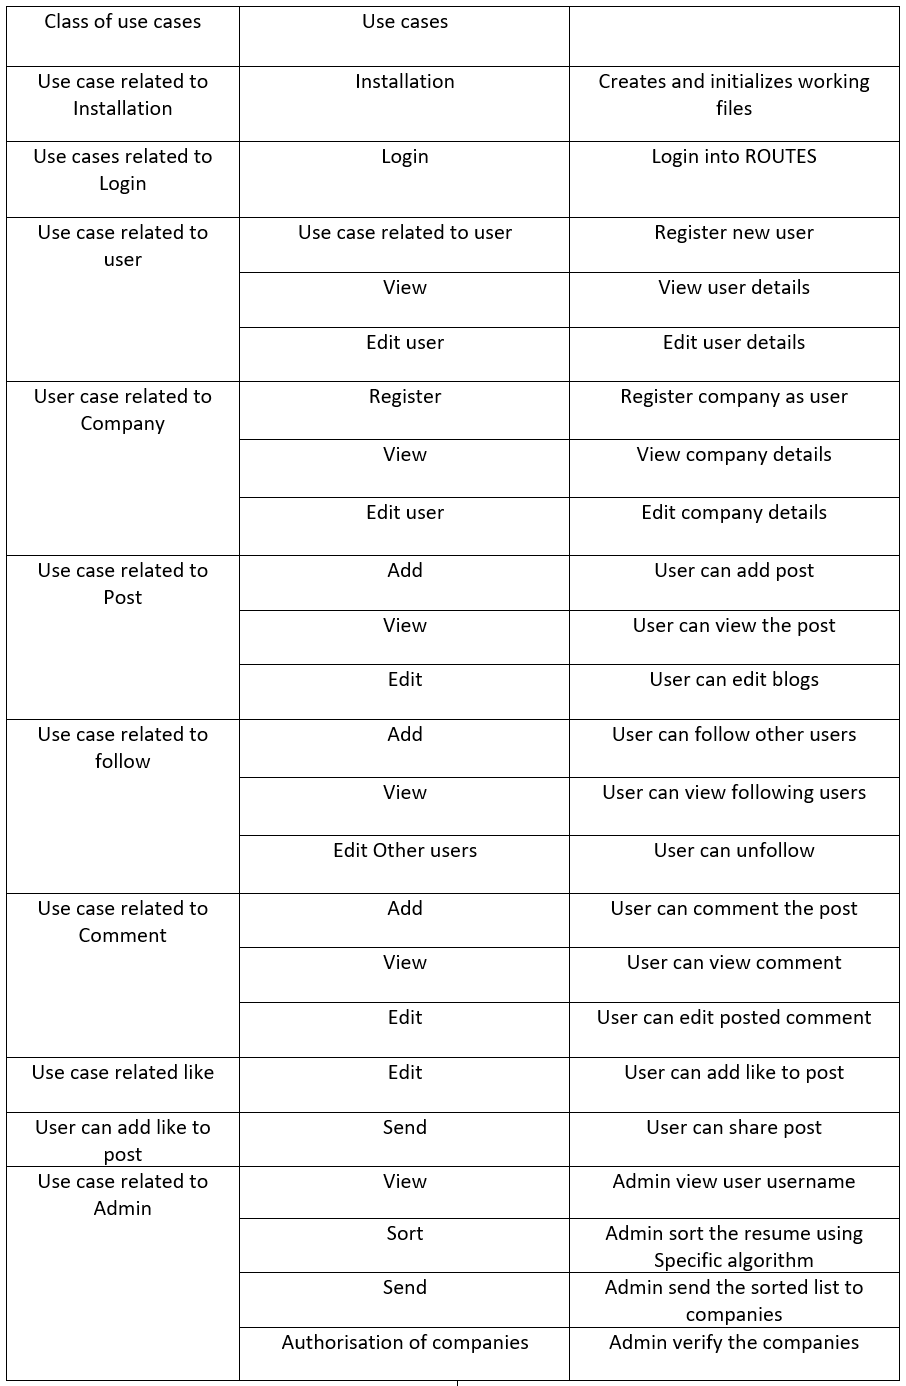
\includegraphics[width=12cm,height=16cm]{fun.png}
		\vspace{.30 cm}
	\end{center}
\end{figure}

\subsection{USER CHARACTERISTICS}
\hspace{01.5cm}This software is going to be used by students,learners,europatours and companies who
browse the net and have Registered themselves at Routes. There are two types of users.
They are Administrator and User.The various functions that can be performed by these
users are indicated in section 3, functional requirements.
\subsection{PRINCIPLE ACTORS}
User Characteristics actors in AD are “User” , “Admin” and “Emergency unit”.
\subsection{GENERAL CONSTRAINTS}
\textbf{1.} It requires minimum internet connection.\\
\textbf{2.} Routes is a multi-user community system.
\subsection{ASSUMPTION AND DEPENDENCIES}
\textbf{1.} Only registered users can use the app.

\section{SPECIFIC REQUIREMENTS}
\subsection{FUNCTIONAL REQUIREMENTS}
\subsubsection{Use case related to Installation}
\textbf{Use Case 1: Installation}\\
Primary Actor: User\\
Pre Condition: Internet connection available.\\
Main Scenario:\\
1. User initiates App installation program.\\
2. System asks the user for the home directory in which all the working files will be created.
Users are also asked for the initial login and password.\\
3. User specifies the home directory and login/password\\
\subsubsection{Use cases related to system login:}
\textbf{Use Case 2: Login}\\
Primary Actor: User\\
Pre Condition: Nil\\
Main Scenario:\\
\begin{figure}[h]
	\begin{center}
		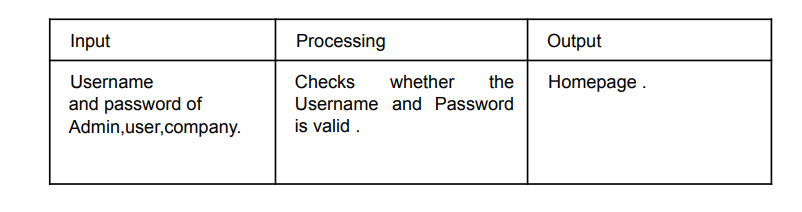
\includegraphics[scale=.90]{tb3.png}
		\vspace{.30 cm}
	\end{center}
\end{figure}\\
\textbf{1.} Start the application. User prompted for login and password.\\
\textbf{2.} User gives the
login and password.\\
\textbf{3.} System does authentication.\\
\textbf{4.} Main screen is displayed.\\
\textbf{Alternate Scenario :}\\
1. 4(a). Authorization fails :\\
a. 4(a)1. Prompt the user that he typed the wrong password\\ b. 4(a)2. Allow him to re-enter
the password. Give him 3 chances.
\\
\\
\subsubsection{Use case related to user}
\textbf{Use Case 3: Registration}\\
Primary Actor: User\\
Pre Condition: Nil\\
Main Scenario:\\
\begin{figure}[h]
	\begin{center}
		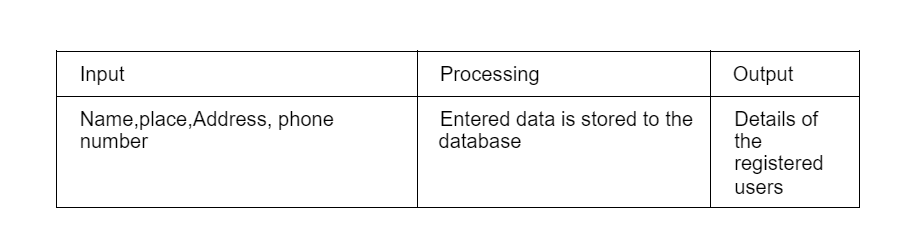
\includegraphics[scale=.80]{tb5.png}
		\vspace{.30 cm}
	\end{center}
\end{figure}\\
1. When user select registration option\\
2. System asks for firstname,lastname,place,post,pin,phone number,username and password
in the first page.\\
3. In the next page the system asks for Educational and Professional details.\\
4. System save data into database\\
5. An alert message shoes “Successfully registered”\\
\\
\textbf{Alternate scenario:}\\
6. Verification fails\\
7. Registration abort\\
\textbf{Use Case 4: View User}\\
Primary Actor:Admin\\
Pre Condition: nil\\
Main Scenario:\\
\begin{figure}[h]
	\begin{center}
		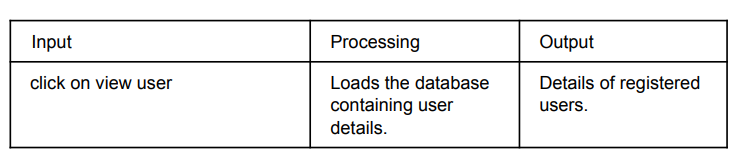
\includegraphics[scale=.90]{tb6.png}
		\vspace{.30 cm}
	\end{center}
\end{figure}\\

1. Admin selects the option of viewing view users\\ 
2. System displays name,address and phone number of the registered users \\
\\
\textbf{Alternate scenario:} \\
1.Database crash \\
\textbf{Use Case 5 : Edit user}\\
Primary Actor:User \\
Pre Condition: Userlogged in\\ 
Main Scenario: \\
\begin{figure}[h]
	\begin{center}
		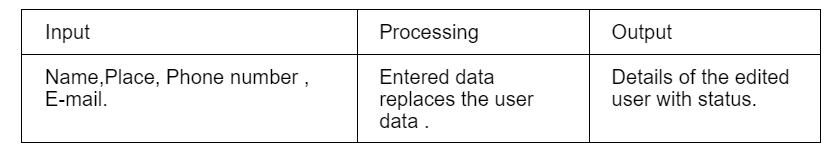
\includegraphics[scale=.90]{tb7.png}
		\vspace{.30 cm}
	\end{center}
\end{figure}\\
1. User select edit option System shows the user info with edit option\\ 2. User can edit details and save \\
3. User details will be edited \\
\textbf{Alternate scenario:}\\
\textbf{Use Case 6: Registration} \\
Primary Actor:User-Company \\
Pre Condition: Nil \\
Main Scenario:\\
\begin{figure}[h]
	\begin{center}
		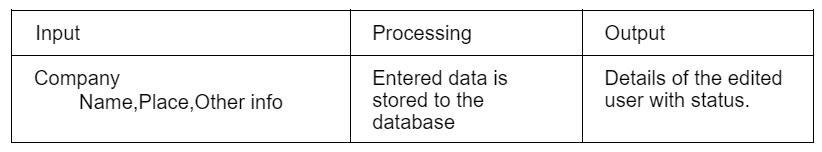
\includegraphics[scale=.90]{tb8.png}
		\vspace{.30 cm}
	\end{center}
\end{figure}\\

\textbf{Alternate scenario:}\\ 
\textbf{Use Case 7: View Company}\\ 
Primary Actor:Admin \\
Pre Condition: nil\\ 
Main Scenario: \\
\begin{figure}[h]
	\begin{center}
		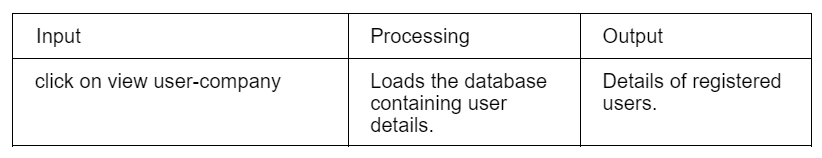
\includegraphics[scale=.90]{tb9.png}
		\vspace{.30 cm}
	\end{center}
\end{figure}\\

1.Admin selects the option of viewing view users \\
2.System displays name,address and phone number of the registered users\\
\textbf{Alternate scenario:} \\
\textbf{Use Case 8 : Edit Company }\\
Primary Actor:User-Company \\
Pre Condition: Userlogged in \\
Main Scenario: \\
\begin{figure}[h]
	\begin{center}
		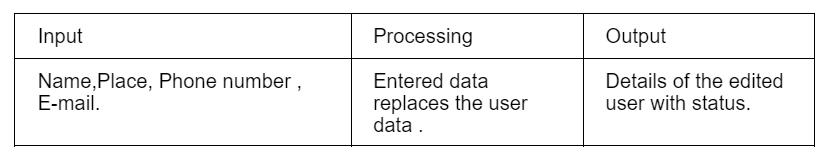
\includegraphics[scale=.90]{tb10.png}
		\vspace{.30 cm}
	\end{center}
\end{figure}\\
1.User select edit option System shows the user info with edit\\ option\\ 2.User can edit details and save\\ 
3.User details will be edited\\
 
\textbf{Alternate scenario:} \\
\subsubsection{Use case related to Notification} 
\textbf{Use Case 9:Send} \\
Primary Actor:Admin \\
Pre Condition: Admin logged in \\
Main Scenario: \\
\begin{figure}[h]
	\begin{center}
		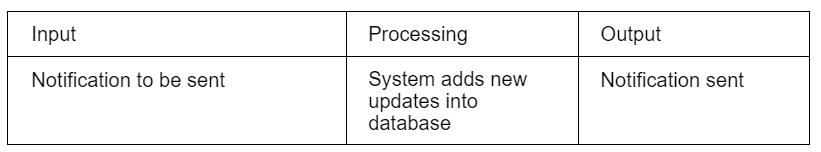
\includegraphics[scale=.90]{tb11.png}
		\vspace{.30 cm}
	\end{center}
\end{figure}\\

\textbf{Use Case 10:View} \\
Primary Actor:User \\
Pre Condition:User logged in \\
Main Scenario: \\
\begin{figure}[h]
	\begin{center}
		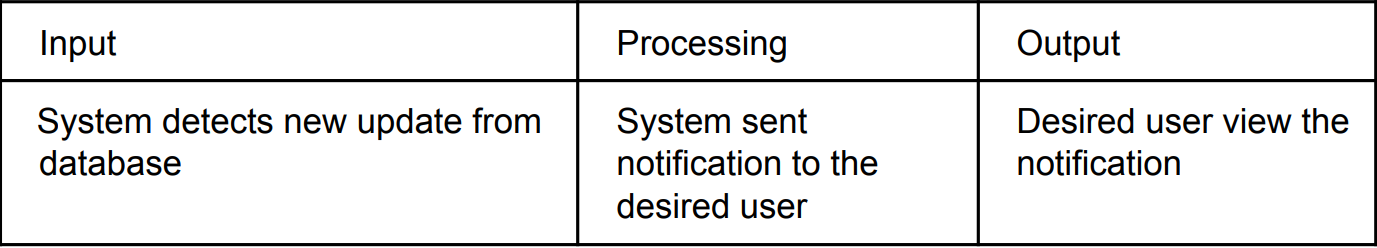
\includegraphics[scale=.43]{tb12.png}
		\vspace{.30 cm}
	\end{center}
\end{figure}\\
1. User must select the notification option in the bottom menu\\
2. System display notifications\\

\textbf{Use Case 11:Add} \\
Primary Actor:User \\
Pre Condition:User logged in \\
Main Scenario: \\
\begin{figure}[h]
	\begin{center}
		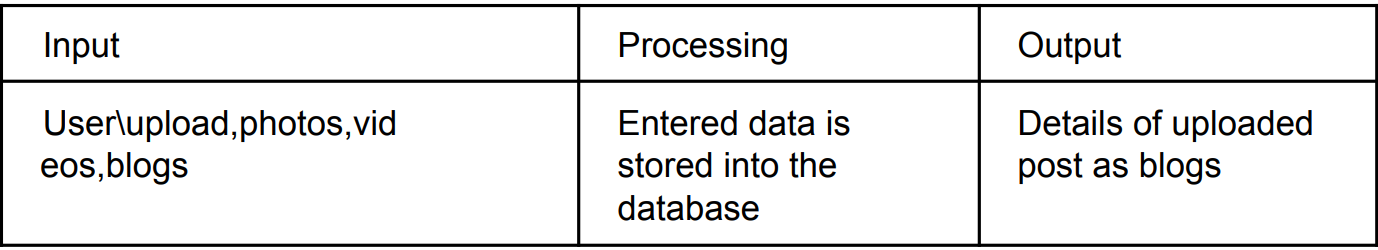
\includegraphics[scale=.43]{tb13.png}
		\vspace{.30 cm}
	\end{center}
\end{figure}\\
1. System adds the data into the database.\\
\textbf{Alternate scenario:} \\

\textbf{Use Case 12:View} \\
Primary Actor:User \\
Pre Condition:User logged in \\
Main Scenario: \\
\begin{figure}[h]
	\begin{center}
		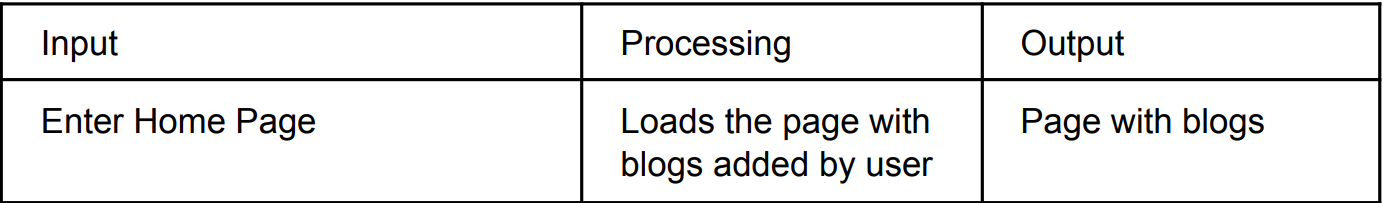
\includegraphics[scale=.43]{tb14.png}
		\vspace{.30 cm}
	\end{center}
\end{figure}\\
\textbf{Alternate scenario:} \\

\textbf{Use Case 13:Edit} \\
Primary Actor:User \\
Pre Condition:User logged in \\
Main Scenario: \\
1. User can add or delete post.\\
2. The added post is viewed in the home page\\
3. User can delete added post from profile.\\
\begin{figure}[h]
	\begin{center}
		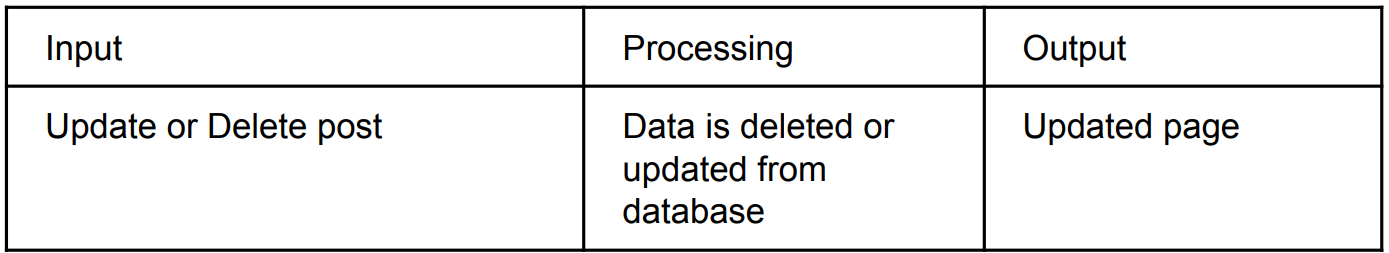
\includegraphics[scale=.43]{tb15.png}
		\vspace{.30 cm}
	\end{center}
\end{figure}\\

\subsubsection{Use case related to Follow }
\textbf{Use Case 14:Add} \\
Primary Actor:User \\
Pre Condition:User logged in \\
Main Scenario: \\
1.User can follow other users.\\
\begin{figure}[h]
	\begin{center}
		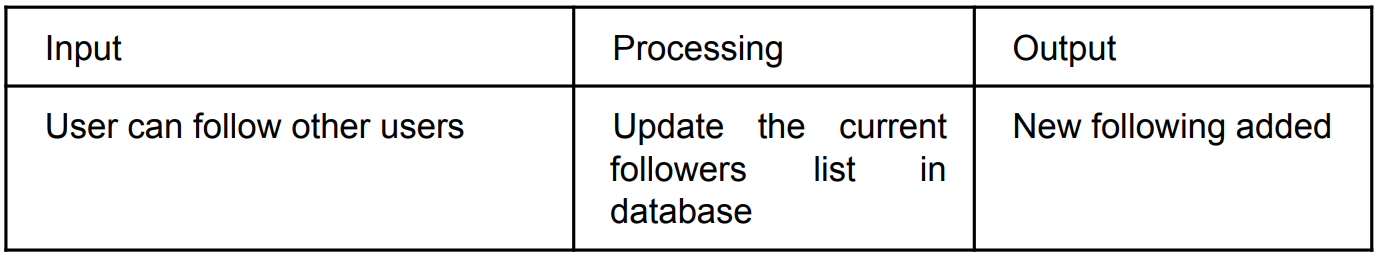
\includegraphics[scale=.43]{tb16.png}
		\vspace{.30 cm}
	\end{center}
\end{figure}\\


\textbf{Use Case 15:View} \\
Primary Actor:User \\
Pre Condition:\\
Main Scenario: \\
1. User can also unfollow others users which is already follows.\\
\begin{figure}[h]
	\begin{center}
		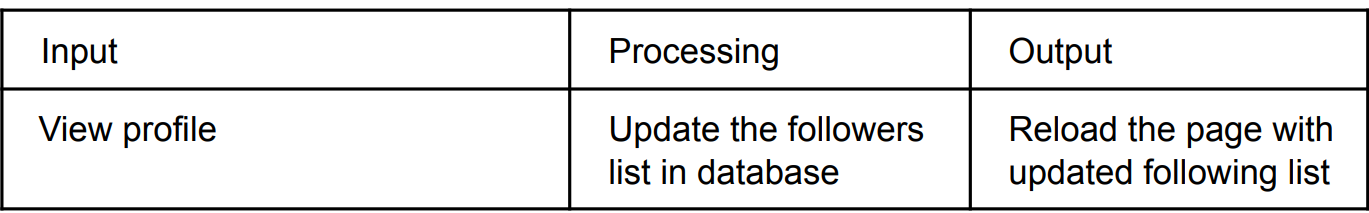
\includegraphics[scale=.43]{tb17.png}
		\vspace{.30 cm}
	\end{center}
\end{figure}\\
\textbf{Alternate scenario:}\\
\textbf{Use case 16:Edit}\\
Primary Actor:\\
Pre Condition:\\
Main Scenario:\\
\begin{figure}[h]
	\begin{center}
		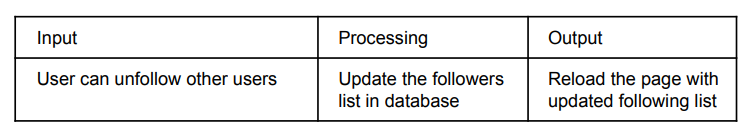
\includegraphics[scale=1]{tb20.png}
		\vspace{.30 cm}
	\end{center}
\end{figure}\\

\textbf{Alternate scenario:}\\
\subsubsection{Use case related to Comment}
\textbf{Use case 17:Add}\\
Primary Actor:User\\
Pre Condition:\\
Main Scenario:
\begin{figure}[h]
	\begin{center}
		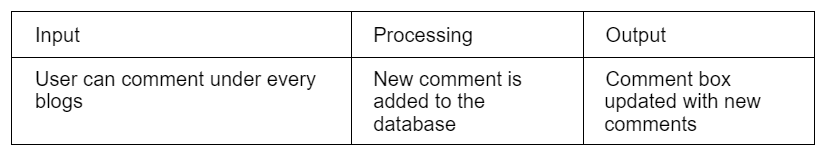
\includegraphics[scale=.90]{tb21.png}
		\vspace{.30 cm}
	\end{center}
\end{figure}\\
\textbf{Alternate scenario:}\\
\textbf{Use case 18:View}\\
Primary Actor:User\\
Pre Condition:user logged in\\
Main Scenario:
\begin{figure}[h]
	\begin{center}
		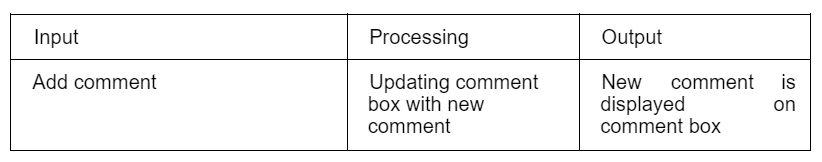
\includegraphics[scale=.90]{tb22.png}
		\vspace{.30 cm}
	\end{center}
\end{figure}\\

\textbf{Alternate scenario:} \\
\textbf{Use case 19:edit }\\
Primary Actor:User \\
Pre Condition: \\
Main Scenario: 
\begin{figure}[h]
	\begin{center}
		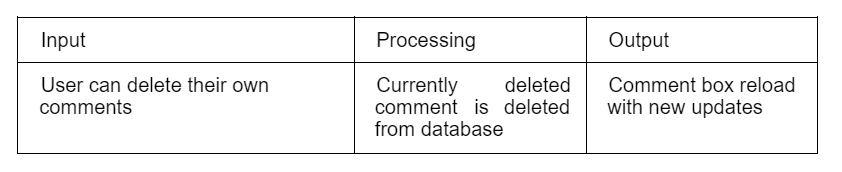
\includegraphics[scale=.90]{tb23.png}
		\vspace{.30 cm}
	\end{center}
\end{figure}\\
\newpage
\subsubsection{Use case related to share }
\textbf{Use case 20:Send }\\
Primary Actor:User \\
Pre Condition: \\
Main Scenario:
\begin{figure}[h]
	\begin{center}
		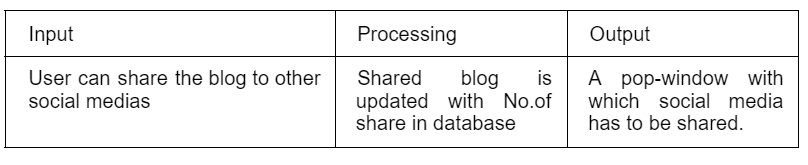
\includegraphics[scale=.90]{tb24.png}
		\vspace{.30 cm}
	\end{center}
\end{figure}\\
\textbf{Alternate scenario: }\\
\subsubsection{Use case related to Like post}
\textbf{Use case 21:Like }\\
Primary Actor:User \\
Pre Condition: \\
Main Scenario: 
\begin{figure}[h]
	\begin{center}
		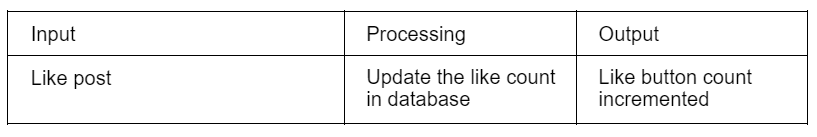
\includegraphics[scale=.90]{tb26.png}
		\vspace{.30 cm}
	\end{center}
\end{figure}\\
\textbf{Alternate scenario:} \\
\textbf{Use case 22:View} \\
Primary Actor:Admin\\ 
Pre Condition: \\
Main Scenario:
\begin{figure}[h]
	\begin{center}
		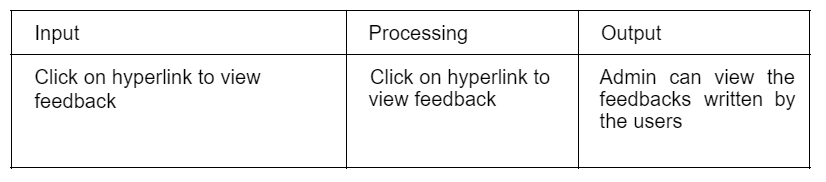
\includegraphics[scale=.90]{tb27.png}
		\vspace{.30 cm}
	\end{center}
\end{figure}\\
\textbf{Alternate scenario:} \\
\subsubsection{Use case related to} Admin
\textbf{Use case 23:View} \\
Primary Actor:Admin\\ 
Pre Condition: \\
Main Scenario: 
\begin{figure}[h]
	\begin{center}
		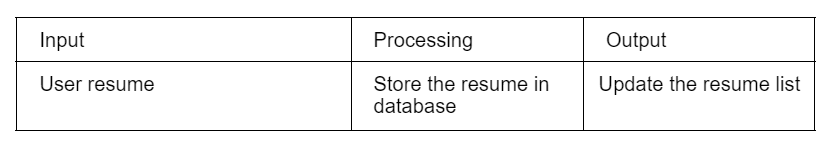
\includegraphics[scale=.90]{tb28.png}
		\vspace{.30 cm}
	\end{center}
\end{figure}\\
\textbf{Use case 24:Sort} \\
Primary Actor:Admin \\
Pre Condition: \\
Main Scenario: 
\begin{figure}[h]
	\begin{center}
		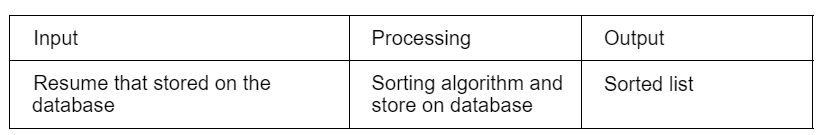
\includegraphics[scale=.90]{tb29.png}
		\vspace{.30 cm}
	\end{center}
\end{figure}\\
\textbf{Use case 25:Send }\\
Primary Actor:Admin \\
Pre Condition: \\
Main Scenario:
\begin{figure}[h]
	\begin{center}
		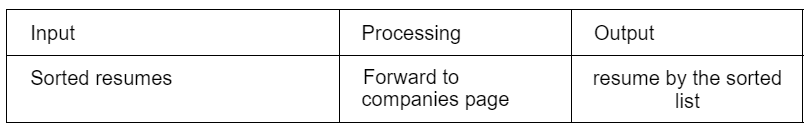
\includegraphics[scale=.90]{tb30.png}
		\vspace{.30 cm}
	\end{center}
\end{figure}

\textbf{Use case 26:Authorisation of companies} \\
Primary Actor:Admin \\
Pre Condition: \\
Main Scenario: 
\begin{figure}[h]
	\begin{center}
		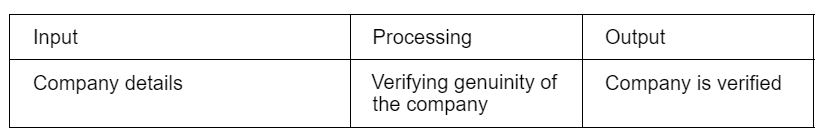
\includegraphics[scale=.90]{tb31.png}
		\vspace{.30 cm}
	\end{center}
\end{figure}

\subsection{ PERFORMANCE REQUIREMENTS}
\subsubsection{HARDWARE AND SOFTWARE REQUIREMENTS}
\textbf{HARDWARE REQUIREMENTS}\\
• Processor : Intel(R) Core(TM) i3-3110M CPU@2.40GHZ(or above)\\
• Memory(RAM) : 4.00 GB \\
• Hard disk : 500 GB\\
• Input devices : Keyboard,touch pad\\
• Output  devices :Monitor,Andriod Phone with basic functionality

\textbf{SOFTWARE REQUIREMENTS}\\
{\bf{ Server Side (Web Application) }}\\
• Frontend : JSP (using Java)\\ 
• Backend : MySQL \\
• Web Server : GlassFish\\ 
• OS : Windows, Mac OS, Linux etc.\\ 
{\bf{Mobile Side}} \\
• Frontend : Flutter\\ 
• Language : Dart\\
• OS : Android/iOs\\ 
• IDE : Visual Studio Code 

\subsubsection{FORNT END}
\textbf{FLUTTER}
\par
\hspace{01.5cm}Flutter, a simple and high performance framework based on Dart language,
provides high performance by rendering the UI directly in the operating system’s
canvas rather than through native framework. The first version of Flutter was known
by the codename ”Sky” and ran on the Android operating system. It was unveiled
at the 2015 Dart developer summit with the stated intent of being able to render
8
consistently at 120 frames per second. During the keynote of Google Developer
Days in Shanghai in September 2018, Google announced Flutter Release Preview
2, which is the last big release before Flutter 1.0. On December 4th of that year,
Flutter 1.0 was released at the Flutter Live event, denoting the first ”stable” version
of the Framework. On December 11, 2019, Flutter 1.12 was released at the Flutter Interactive event. On May 6, 2020, the Dart software development kit (SDK)
in version 2.8 and the Flutter in version 1.17.0 were released, where support was
added to the Metal API, improving performance on iOS devices (approximately
50%), new Material widgets, and new network tracking.
\par
On March 3, 2021, Google released Flutter 2 during an online Flutter Engage event. This major update brought official support for web-based applications
with new CanvasKit renderer and web specific widgets, early-access desktop application support for Windows, macOS, and Linux and improved Add-to-App APIs.
This release included sound null-safety, which caused many breaking changes and
issues with many external packages, but the Flutter team included instructions to
mitigate these changes as well. On September 8th, 2021, the Dart SDK in version
2.14 and Flutter version 2.5 were released by Google. The update brought improvements to the Android Full-Screen mode and the latest version of Google’s Material
Design called Material You. Dart received two new updates, the newest lint conditions have been standardized and preset as the default conditions as well Dart for
Apple Silicon is now stable.\\
\textbf{ADVANTAGES}\\
1. Large Community Support\\
2. Faster Code Writing\\
3. Own Rendering Engine\\
4. Cross Platform\\
5. Rich Libraries\\
6. Fast testing with hot reload\\

\textbf{DART}\\
\hspace{01.5cm}Dart is a general-purpose, high-level modern programming language which
is originally developed by Google. It is the new programming language which is
emerged in 2011, but its stable version was released in June 2017. Dart is a dynamic, class-based, object-oriented programming language with closure and lexical scope. Syntactically, it is quite similar to Java, C, and JavaScript. Dart is an
open-source programming language which is widely used to developthe mobile application, modern web-applications, desktop application, and the Internet of Things
(IoT) using by Flutter framework.\\


\textbf{JAVA}\\
\hspace{01.5cm}Java was originally developed by James Gosling at Sun Microsystems and
released in May 1995 as a core component of Sun Microsystems’ Java platform.
The original and reference implementation Java compilers, virtual machines, and
class libraries were originally released by Sun under proprietary licenses.
Principles
There were five primary goals in the creation of the Java language:
1. It must be simple, object-oriented, and familiar.\\
2. It must be robust and secure.\\
3. It must be architecture-neutral and portable.\\
4. It must execute with high performance.\\
5. It must be interpreted, threaded, and dynamic.
\\
\subsubsection{IDE}
\textbf{VISUAL STUDIO CODE}\\
\hspace{01.5cm}Visual Studio Code, also commonly referred to as VS Code, is a sourcecode editor made by Microsoft for Windows, Linux and macOS. Features include
support for debugging, syntax highlighting, intelligent code completion, snippets,
code refactoring, and embedded Git. Users can change the theme, keyboard shortcuts, preferences, and install extensions that add additional functionality. In the
Stack Overflow 2021 Developer Survey, Visual Studio Code was ranked the most
popular developer environment tool, with 70% of 82,000 respondents reporting that
10
they use it.
Visual Studio Code was first announced on April 29, 2015, by Microsoft
at the 2015 Build conference. A preview build was released shortly thereafter. On
November 18, 2015, the source of Visual Studio Code was released under the MIT
License, and made available on GitHub. Extension support was also announced.
On April 14, 2016, Visual Studio Code graduated from the public preview stage
and was released to the Web. Microsoft has released most of Visual Studio Code’s
source code on GitHub under the permissive MIT License, while the releases by
Microsoft are proprietary freeware.
\\
\textbf{NetBeans IDE}\\
\hspace{01.5cm}NetBeans IDE is a free and open source integrated development environment for application development on Windows, Mac, Linux, and Solaris operating
systems.The IDE simplifies the development of web, enterprise, desktop, and mobile applications that use the Java and HTML5 platforms. The IDE also offers
support for the development of PHP and C/C++ applications.
NetBeans IDE offers first-class tools for Java web, enterprise, desktop,
and mobile application development. It is consistently the first IDE to support the
latest versions of the JDK, Java EE, and JavaFX. It provides smart overviews to
help you understand and manage your applications, including ouf-of-the-box support for popular technologies such as Maven.
With its end-to-end application development features, constantly improving Java Editor, and continual speed and performance enhancements, NetBeans
IDE sets the standard for application development with cutting edge technologies
out of the box.\\

\subsubsection{BACK END}
\textbf{MySQL}\\
\hspace{01.5cm}MySQL is a relational database management system (RDBMS) developed
by Oracle that is based on structured query language (SQL).
A database is a structured collection of data. It may be anything from a
simple shopping list to a picture gallery or a place to hold the vast amounts of information in a corporate network. In particular, a relational database is a digital store
collecting data and organizing it according to the relational model. In this model,
tables consist of rows and columns, and relationships between data elements all follow a strict logical structure. An RDBMS is simply the set of software tools used
to actually implement, manage, and query such a database.
MySQL is integral to many of the most popular software stacks for building and maintaining everything from customer-facing web applications to powerful, data-driven B2B services. Its open-source nature, stability, and rich feature
set, paired with ongoing development and support from Oracle, have meant that
internet-critical organizations such as Facebook, Flickr, Twitter, Wikipedia, and
YouTube all employ MySQL backends.
In a simple manner, SQL is a non-procedural, English-like language that
processes data in groups of records rather than one record at a time.
\subsubsection{WHY SQL USED IN THIS SYSTEM}
\hspace{01.5cm}SQL server can be used to develop both simple and complex database. Its wonderfully designed built-in wizard makes allow look like a product that any one can use. Although it is true that the simplest of the access application can be produced without any thought of design and without a single line of code written by the user, most applications require at least some designing and customer codes. It can store more data. So I used it in my project

\subsection{ NON-FUNCTIONAL REQUIREMENTS}
\hspace{01.5cm}Non-Functional requirements are the constraints or the requirements im-posed on the system. They specify the quality attribute of the software.\\
\subsubsection{SECURITY }
\hspace{01.5cm}The system need to store the data in a secure location and store in a secure format. It requires a secure communication channel for the data, and the system needs to control the system’s sessions.\\
\subsubsection{CONCURRENCY and CAPACITY  }
\hspace{01.5cm}System should be able to recruit employees and helps the jobseekers to find dream job based on their skill and experience and potentially interacting with employees and employers.\\
\subsubsection{ PERFORMANCE}
\hspace{01.5cmThe performance of recruiting process of the system is depending on the accuracy in skill and experience of the jobseekers. We are using K-means algorithm which reaps an accuracy of 78.33 percentage}\\
\subsubsection{ RELIABILITY}
\hspace{01.5cm}It is necessary to ensure and verify the systems reliability for our ROUTES system. We should use powerful RDBMS system, such as MySQL, to make the data secure from system crashes. This makes the system highly reliable.\\
\subsubsection{MAINTAINABILITY}
\hspace{01.5cm}The system need to be regularly checked for preventive and corrective maintenance as it would come up with addition feature requirements or removing undesired events. Maintenance might specify scalability to grow and improve the system features and functionalities\\
\subsubsection{ USABILITY}
\hspace{01.5cm}End user satisfaction and acceptance is one of the key pillars that support a project success. As we are using Flutter framework, we can implement a simple yet powerful system and thereby it enhances the system usability\\

\subsection{ DESIGN CONSTRAINTS }
\subsubsection{RISK OF IDENTITY THEFT}
\hspace{01.5cm}There are loads of personal information that you have to display on your profile for prospective employers.\\
\subsubsection{ATTRACTS BAD CANDIDATES}
\hspace{01.5cm}As previously mentioned, it’s very easy for people to apply for jobs online; this can potentially be a negative point as well, though. Posting a position online usually results in hundreds of applicants, many of whom will not be suitable for or serious about the role, thus diluting the quality of your talent pool.\\
\subsubsection{ATTRACTS FRAUDULENT APPLICANTS}
\hspace{01.5cm}Some applications might be fake to get information about the company or hiring officer (a common espionage tactic). Simultaneously, spammers might use the information posted online to promote a service or product to your company.\\
\subsection{ FUTURE EXTENSIONS }
\hspace{01.5cm}We can add more interactive session for user and company by providing live events and challanges. Using cloud storage system can improve reliability and performance. Features like suggestions, notifications, etc can be added. Two step verification of accounts can be added for enhanced privacy . Privacy can be reaped by privatization of user profile.\\
\chapter{SYSTEM DESIGN}
\section{MODULE DESCRIPTION}
\hspace{01.5cm}The complete project is divided into two modules. And the modularization is based on the type of the users in the system. The different modules based on the type of the users of the system are:\\
\textbf{1.}User module\\
\textbf{2.}Company module\\
\subsection{NORMAL USER}
\textbf{1.}Create a new account\\
\textbf{2.}Add ,view and delete post\\
\textbf{3.}Add,view and delete comments\\
\textbf{4.}Save Post and view saved post\\
\textbf{5.}Follow an account\\
\textbf{6.}Like and unlike a post\\
\textbf{7.}Apply for a job
\subsection{COMPANY USER}
\textbf{1.}Create a new account\\
\textbf{2.}Add ,view and delete post\\
\textbf{3.}Add,view and delete comments\\
\textbf{4.}Save Post and view saved post\\
\textbf{5.}Follow an account\\
\textbf{6.}Like and unlike a post\\
\textbf{7.}Add  new job applications\\
\section{DATABASE DESIGN}
\begin{figure}[h]
	\begin{center}
		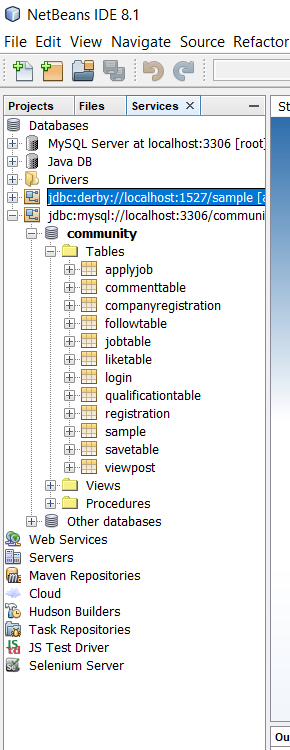
\includegraphics[scale=1]{t1.png}
		\caption{TABLES}
	\end{center}
\end{figure}
\newpage
\begin{figure}[h]
	\begin{center}
		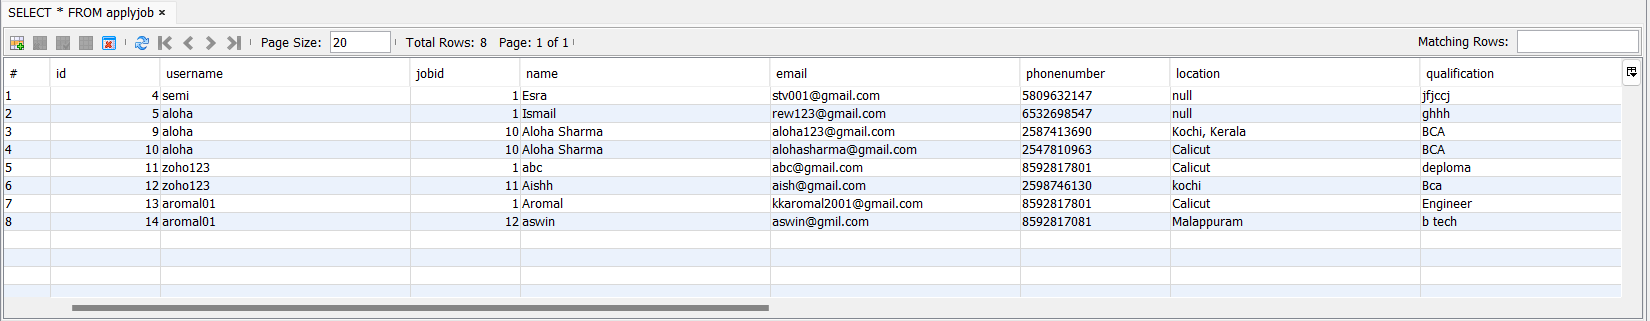
\includegraphics[scale=.40]{t2.png}
		\caption{LOGIN TABLE(USER AND COMPANY)}
	\end{center}
\end{figure}
\begin{figure}[h]
	\begin{center}
		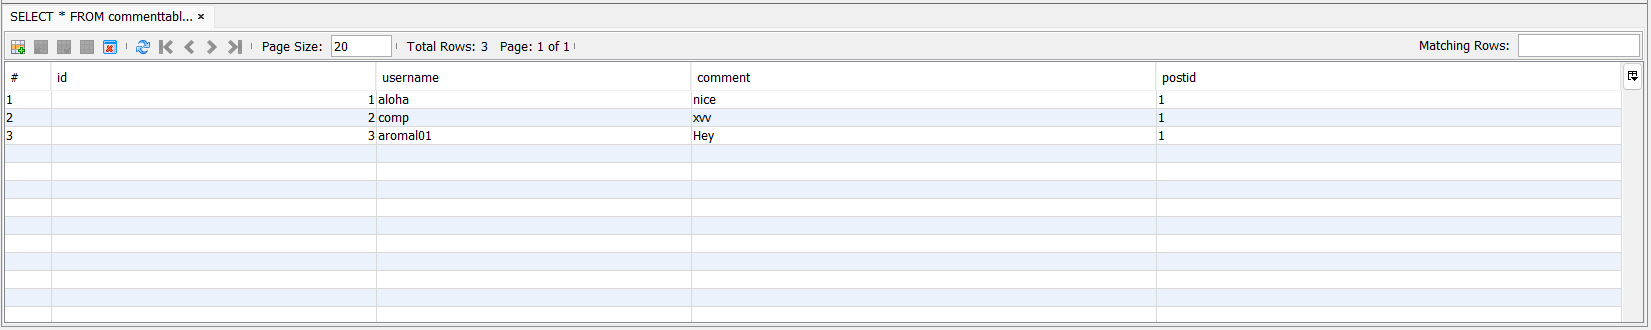
\includegraphics[scale=.40]{3.png}
		\caption{USER LOGIN ONLY}
	\end{center}
\end{figure}
\begin{figure}[h]
	\begin{center}
		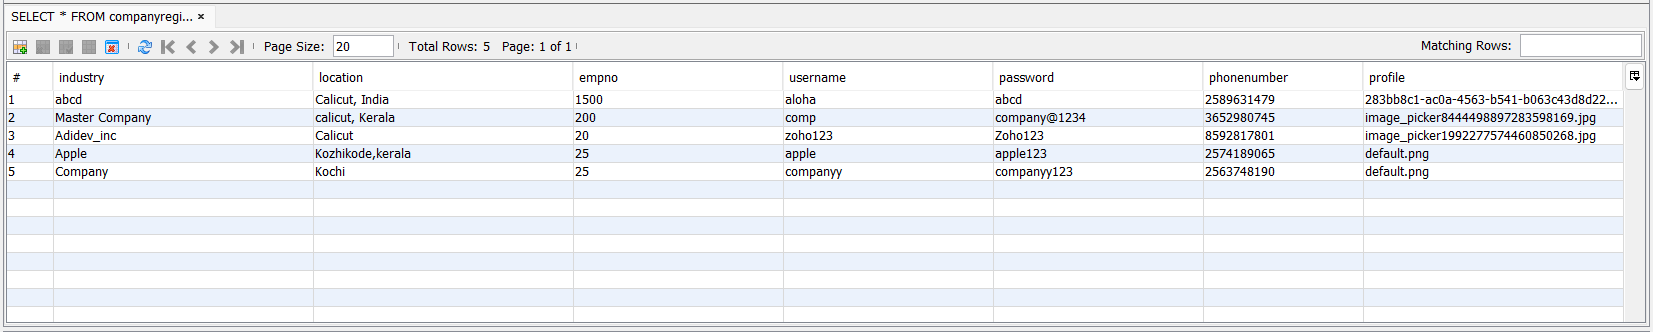
\includegraphics[scale=.40]{4.png}
		\caption{LOGIN TABLE(USER AND COMPANY)}
	\end{center}
\end{figure}
\begin{figure}[h]
	\begin{center}
		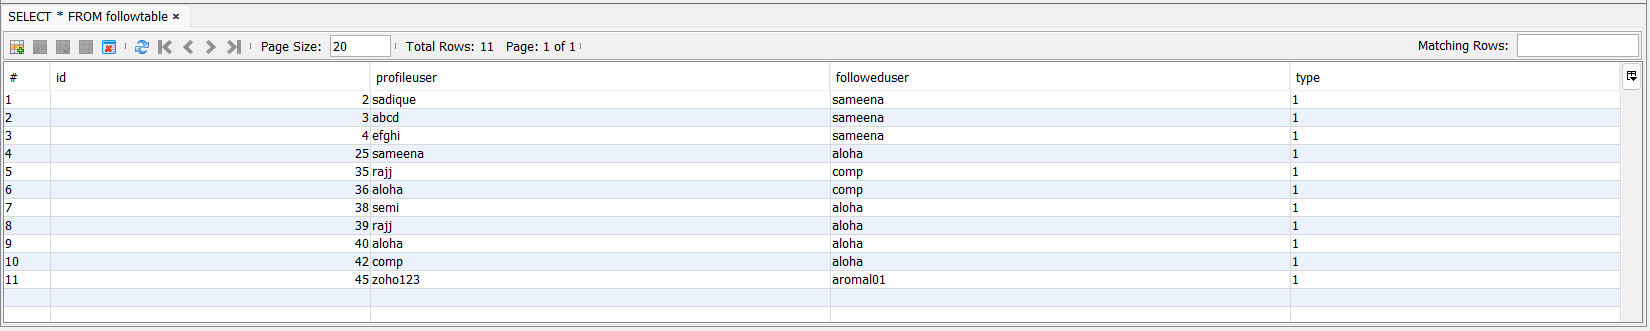
\includegraphics[scale=.40]{5.png}
		\caption{USER LOGIN ONLY}
	\end{center}
\end{figure}
\begin{figure}[h]
	\begin{center}
		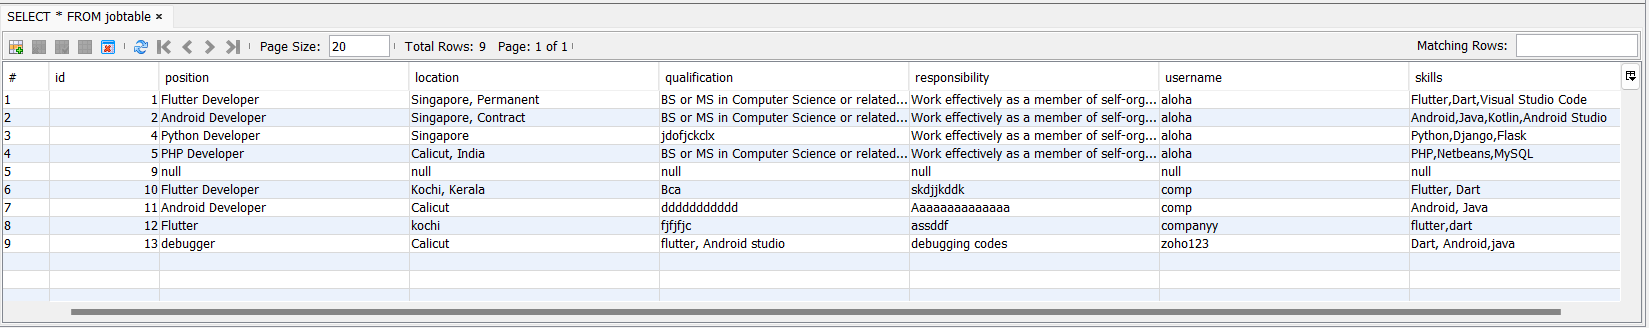
\includegraphics[scale=.40]{6.png}
		\caption{LOGIN TABLE(USER AND COMPANY)}
	\end{center}
\end{figure}

\newpage
\section{DATA FLOW DIAGRAM}
\subsection{LEVEL 0}
\begin{figure}[h]
	\begin{center}
		\fbox{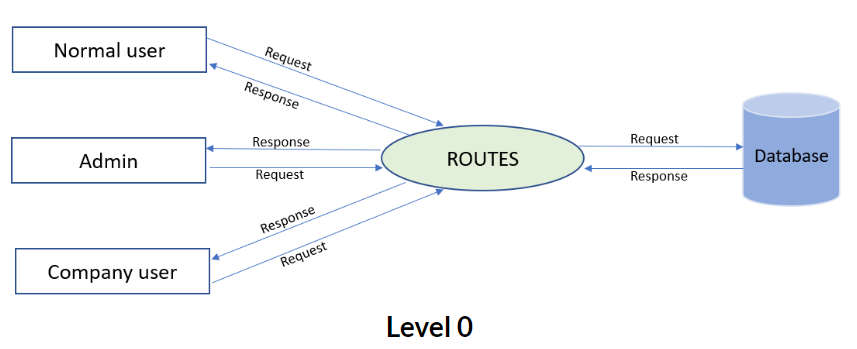
\includegraphics[scale=.60]{dfd01.png}}
		\caption{Level 0}
	\end{center}
\end{figure}
\newpage
\subsection{LEVEL 1}
\begin{figure}[h]
	\begin{center}
		\fbox{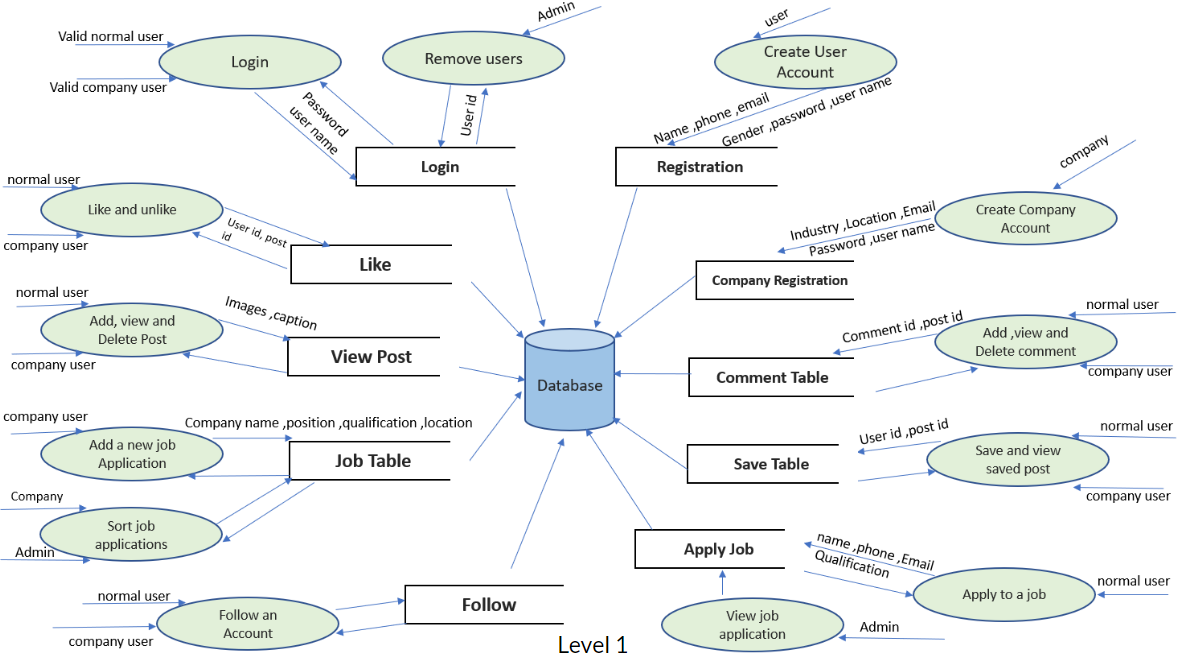
\includegraphics[scale=.52]{dfd02.png}}
		\caption{Level 1}
	\end{center}
\end{figure}
\newpage
\section{FORM DESIGN}
\subsection{ Mobile UI }
\begin{figure}[h]
	\begin{center}
		\fbox{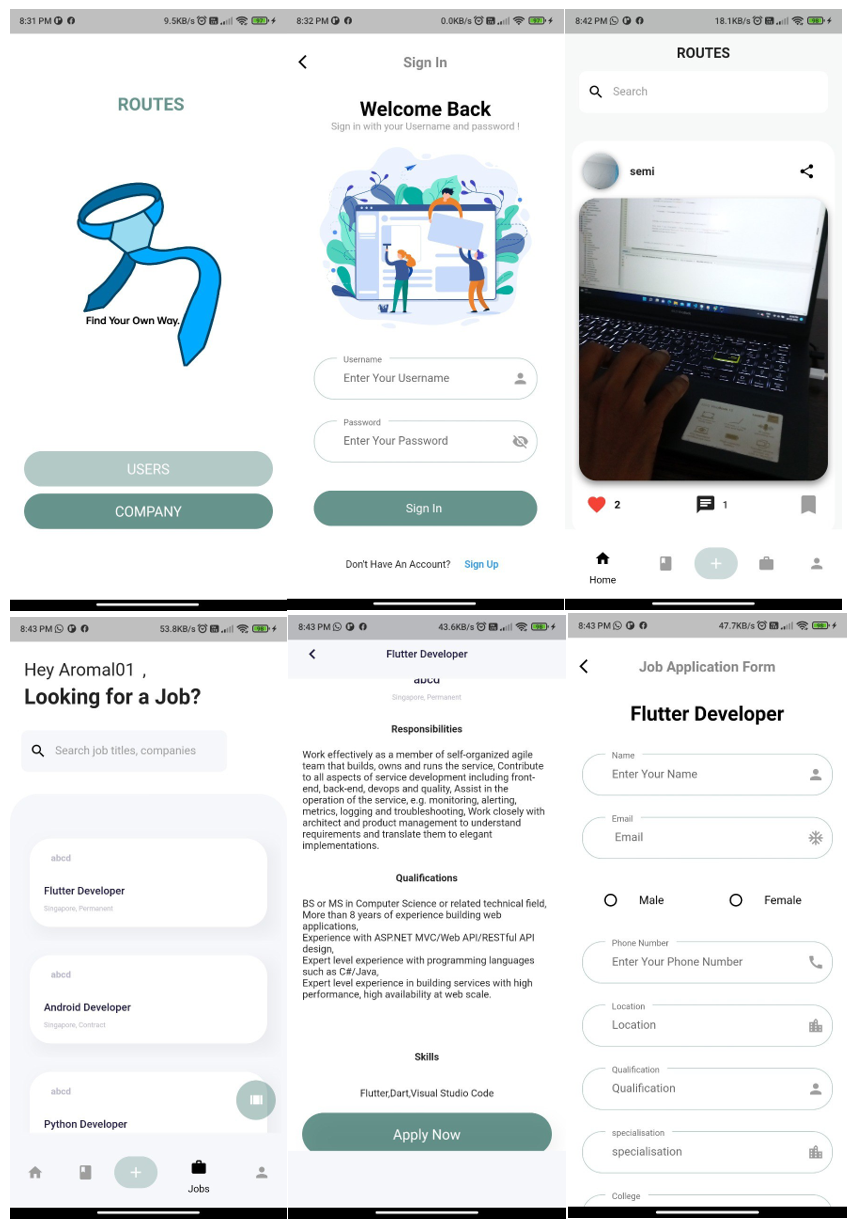
\includegraphics[scale=.50]{1.png}}
		\caption{Mobile user interfaces}
	\end{center}
\end{figure}
\newpage
\subsection{ Web UI }
\begin{figure}[h]
	\begin{center}
		\fbox{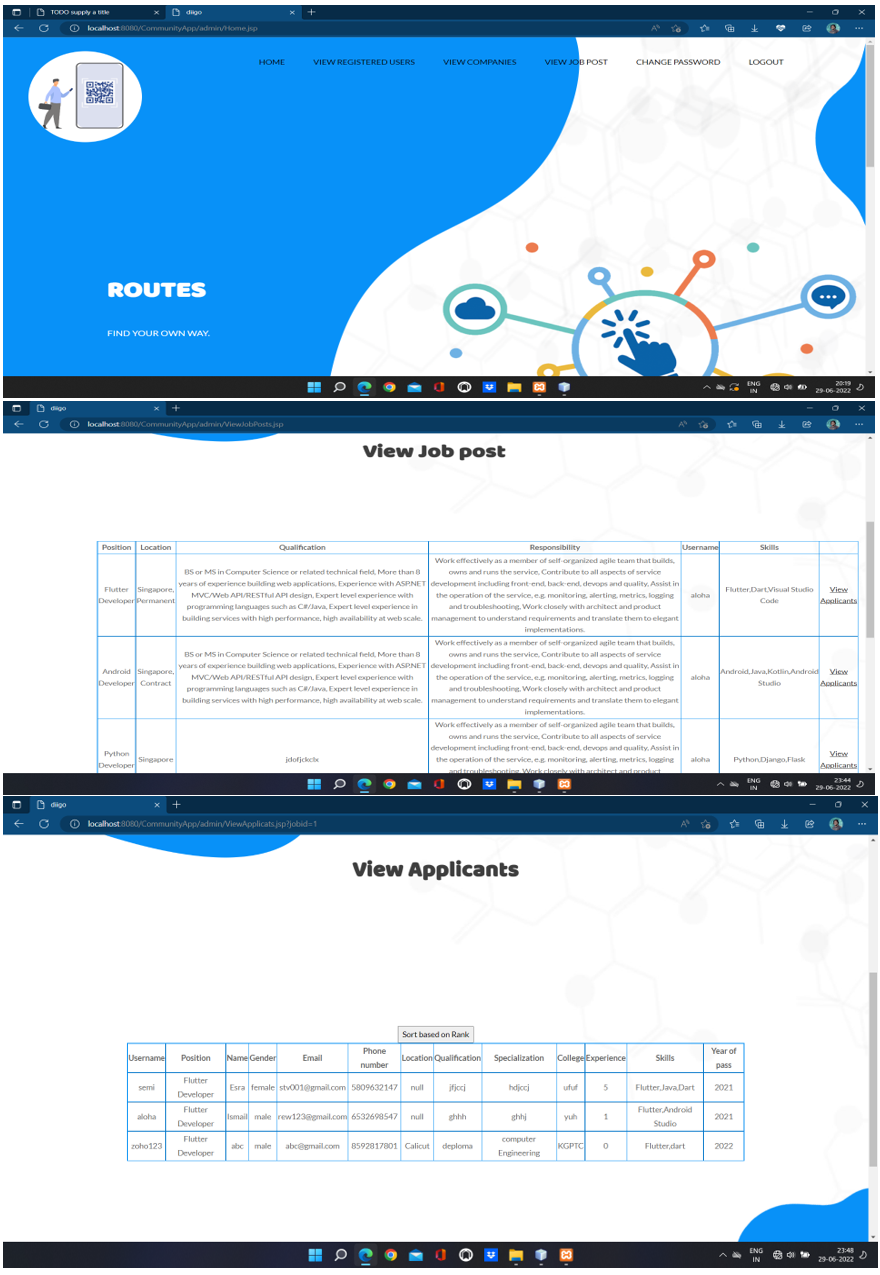
\includegraphics[scale=.50]{2.png}}
		\caption{Web user interfaces}
	\end{center}
\end{figure}
\chapter{SYSTEM IMPLEMENTATION AND RESULT}
\section{ Important Codes}
\subsection{ Log in(loginModel.dart)}
\begin{lstlisting}
class loginModel {
  final String username;
  final String password;
  final String type;
  loginModel({this.username, this.password, this.type});
  factory loginModel.fromJson(Map<String, dynamic> Json) {
    return loginModel(
        username: Json['username'],
        password: Json['password'],
        type: Json['type']);
  }
}
\end{lstlisting}

\subsection{Sign up (registrationModel.dart)}
\begin{lstlisting}
class regModel {
  final String id;
  final String name;
  final String rollnoOrEmpno;
  final String college;
  final String phonenumber;
  final String username;
  final String password;
  final String gender;
  regModel(
      {this.id,
      this.name,
      this.rollnoOrEmpno,
      this.college,
      this.phonenumber,
      this.username,
      this.password,
      this.gender});
  factory regModel.fromJson(Map<String, dynamic> Json) {
    return regModel(
        id: Json['id'],
        name: Json['name'],
        rollnoOrEmpno: Json['rollnoOrEmpno'],
        college: Json['college'],
        phonenumber: Json['phonenumber'],
        username: Json['username'],
        password: Json['password'],
        gender: Json['gender']);
  }
}
\end{lstlisting}

\subsection{ Add Job (jobDetailsModel.dart)}
\begin{lstlisting}
class JobModel {
  final String id;
  // final String companylogo;
  final String industry;
  final String position;
  final String location;
  final String responsibility;
  final String qualification;
  final String skills;
  JobModel({
    this.id,
    // this.companylogo,
    this.industry,
    this.position,
    this.location,
    this.qualification,
    this.responsibility,
    this.skills
  });
  factory JobModel.fromJson(Map<String, dynamic> Json) {
    print((Json['id']));
    print((Json['industry']));
    print((Json['position']));
    print((Json['location']));
    print((Json['responsibility']));
    print((Json['qualification']));
    print((Json['skills']));
    try {
      return JobModel(
        id: Json['id'],
        // companylogo: Json['companylogo'],
        industry: Json['industry'],
        position: Json['position'],
        location: Json['location'],
        responsibility: Json['responsibility'],
        qualification: Json['qualification'],
        skills: Json['skills']
      );
    } catch (error) {
      print(error);
    }
  }
}
\end{lstlisting}

\subsection{ Post (viewPostModel.dart)}
\begin{lstlisting}
class ViewpostModel {
  final String id;
  final String username;
  final String userimage;
  final String image;
  final String post_title;
  final String post_contenct;
  final String date;
  final String likecount;
  final String profile;
  ViewpostModel(
      {this.id,
      this.username,
      this.userimage,
      this.image,
      this.post_title,
      this.post_contenct,
      this.date,
      this.likecount,
      this.profile
      });
  factory ViewpostModel.fromJson(Map<String, dynamic> Json) {
    print((Json['id']));
    print((Json['username']));
    print((Json['userimage']));
    print((Json['image']));
    print((Json['post_title']));
    print((Json['post_contenct']));
    print((Json['date']));
    print((Json['likecount']));
    print((Json['profile']));
    try {
      return ViewpostModel(
        id: Json['id'],
        username: Json['username'],
        userimage: Json['userimage'],
        image: Json['image'],
        post_title: Json['post_title'],
        post_contenct: Json['post_contenct'],
        date: Json['date'],
        likecount: Json['likecount'],
        profile: Json['profile']
      );
    } catch (error) {
      print(error);
    }
  }
}
\end{lstlisting}

\subsection{ Apply job (applyjobsuccessModell.dart)}
\begin{lstlisting}
class JobSuccessModel {
  final String username;
  final int jobid;
  final String position;
  final String name;
  final String gender;
  final String email;
  final String location;
  final String phonenumber;
  final String qualification;
  final String specialisation;
  final String college;
  final String experience;
  final String skills;
  final String yearofpass;
  JobSuccessModel(
      {this.username,
      this.position,
      this.jobid,
      this.name,
      this.gender,
      this.email,
      this.college,
      this.experience,
      this.phonenumber,
      this.location,
      this.qualification,
      this.skills,
      this.specialisation,
      this.yearofpass});
  factory JobSuccessModel.fromJson(Map<String, dynamic> Json) {
    return JobSuccessModel(
        username: Json['username'].toString(),
        jobid: Json['jobid'],
        position: Json['position'].toString(),
        name: Json['name'].toString(),
        gender: Json['gender'].toString(),
        email: Json['email'].toString(),
        phonenumber: Json['phonenumber'].toString(),
        location: Json['location'].toString(),
        qualification: Json['qualification'].toString(),
        specialisation: Json['specialisation'].toString(),
        college: Json['college'].toString(),
        experience: Json['experience'].toString(),
        skills: Json['skills'].toString(),
        yearofpass: Json['yearofpass'].toString());
  }
}
\end{lstlisting}


\section{ KMeans Clustering.java}
\begin{lstlisting}
package com.packages;
import java.util.ArrayList;
import java.util.Vector;
public class KMeans_Clustering {
    public static final int NUM_CLUSTERS = 5;    // Total clusters.
    public static int TOTAL_DATA = 5;      // Total data points.
    private static double SAMPLES[][] = new double[][]{{1.0, 3.8},
    {4.2, 5.0},
    {5.6, 6.0},
    {6.8, 7.0},
    {7.2, 9.0},};
    Vector v = null;
    String type = "", sql = "";
    Vector studentsinCluster = new Vector();
    DBConnection db = null;
    public KMeans_Clustering(Vector dataset, String type)
{//argument constructor
        v = dataset;
        TOTAL_DATA = v.size();
        this.type = type;
        db = new DBConnection();
    }
    public ArrayList<Data> dataSet = new ArrayList<Data>();
    private ArrayList<Centroid> centroids = 
new ArrayList<Centroid>();
    private void initialize() {
        System.out.println("Centroids initialized at:");
 centroids.add(new Centroid(70.1, 100.0)); // Excellent.
 centroids.add(new Centroid(60.51, 70.0)); // Good.
 centroids.add(new Centroid(50.51, 60.50)); // Average.
centroids.add(new Centroid(40.51, 50.50)); // Below Average.
centroids.add(new Centroid(1, 40.5)); // Need Improvement.
System.out.println("     (" + centroids.get(0).X() + ",
" + centroids.get(0).Y() + ")");
System.out.println("     (" + centroids.get(1).X() + ",
 " + centroids.get(1).Y() + ")");
System.out.print("\n");
return;
    }
    private void kMeanCluster() {
        final double bigNumber = Math.pow(10, 10);  
        double minimum = bigNumber;                  
        double distance = 0.0;                      
        int sampleNumber = 0;
        int cluster = 0;
        boolean isStillMoving = true;
        Data newData = null;
        StScoreBean bean = null;
        while (dataSet.size() < TOTAL_DATA) Z
            bean = (StScoreBean) v.get(sampleNumber);
            double score = 0;
            double minScore = 0;
            System.out.println("score ::" + score);
            if (type.equals("overall")) {
                score = bean.getTotalscore();
                minScore = bean.getScore_min_range();
                sql="UPDATE applyjob set totalscore=
	"+bean.getTotalscore()+" , review='"+bean.getRank()+
	"' where username='"+bean.username+"' and jobid=
	"+bean.jobid+"";
                System.out.println(sql);
                db.executeSQL(sql);
            } 
            System.out.println("score after :: " + score);          
            newData = new Data(minScore, score, bean);
            dataSet.add(newData);
            minimum = bigNumber;
            for (int i = 0; i < NUM_CLUSTERS; i++) { 
                distance = dist(newData, centroids.get(i));
                if (distance < minimum) {
                    minimum = distance;
                    cluster = i;
                }
            }
            newData.cluster(cluster);
            // calculate new centroids.
            for (int i = 0; i < NUM_CLUSTERS; i++) {
                int totalX = 0;
                int totalY = 0;
                int totalInCluster = 0;
                for (int j = 0; j < dataSet.size(); j++) {
                    if (dataSet.get(j).cluster() == i) {
                        totalX += dataSet.get(j).X();
                        totalY += dataSet.get(j).Y();
                        totalInCluster++;
                    }
                }
                if (totalInCluster > 0) {
                    centroids.get(i).X(totalX / totalInCluster);
                    centroids.get(i).Y(totalY / totalInCluster);
                }
            }
            sampleNumber++;
        }
        // Now, keep shifting centroids until equilibrium occurs.
        while (isStillMoving) {
            // calculate new centroids.
            for (int i = 0; i < NUM_CLUSTERS; i++) {
                int totalX = 0;
                int totalY = 0;
                int totalInCluster = 0;
                for (int j = 0; j < dataSet.size(); j++) {
                    if (dataSet.get(j).cluster() == i) {
                        totalX += dataSet.get(j).X();
                        totalY += dataSet.get(j).Y();
                        totalInCluster++;
                    }
                }
                if (totalInCluster > 0) {
                    centroids.get(i).X(totalX / totalInCluster);
                    centroids.get(i).Y(totalY / totalInCluster);
                }
            }
            // Assign all data to the new centroids
            isStillMoving = false;

            for (int i = 0; i < dataSet.size(); i++) {
                Data tempData = dataSet.get(i);
                minimum = bigNumber;
                for (int j = 0; j < NUM_CLUSTERS; j++) {
                    distance = dist(tempData, centroids.get(j));
                    if (distance < minimum) {
                        minimum = distance;
                        cluster = j;
                    }
                }
                tempData.cluster(cluster);
                if (tempData.cluster() != cluster) {
                    tempData.cluster(cluster);
                    isStillMoving = true;
                }
            }
        }
        return;
    }
    /**
     * // Calculate Euclidean distance.
     *
     * @param d - Data object.
     * @param c - Centroid object.
     * @return - double value.
     */
    private static double dist(Data d, Centroid c) {
        return Math.sqrt(Math.pow((c.Y() - d.Y()), 2)
 + Math.pow((c.X() - d.X()), 2));
    }
    public static class Data {
        public double mX = 0;
        public double mY = 0;
        public int mCluster = 0;
        private StScoreBean jobseekerbean;
        /**
         * Get the value of studentbean
         *
         * @return the value of studentbean
         */
        public StScoreBean getStudentbean() {
            return jobseekerbean;
        }
        /**
         * Set the value of studentbean
         *
         * @param studentbean new value of studentbean
         */
        public void setStudentbean(StScoreBean studentbean) {
            this.jobseekerbean = studentbean;
        }
        public Data() {
            return;
        }
        public Data(double x, double y, StScoreBean bean) {
            this.X(x);
            this.Y(y);
            this.jobseekerbean = bean;
            return;
        }
        public void X(double x) {
            this.mX = x;
            return;
        }
        public double X() {
            return this.mX;
        }
        public void Y(double y) {
            this.mY = y;
            return;
        }
        public double Y() {
            return this.mY;
        }
        public void cluster(int clusterNumber) {
            this.mCluster = clusterNumber;
            return;
        }
        public int cluster() {
            return this.mCluster;
        }
    }
    private static class Centroid {
        private double mX = 0.0;
        private double mY = 0.0;
        public Centroid() {
            return;
        }
        public Centroid(double newX, double newY) {
            this.mX = newX;
            this.mY = newY;
            return;
        }
        public void X(double newX) {
            this.mX = newX;
            return;
        }
        public double X() {
            return this.mX;
        }
        public void Y(double newY) {
            this.mY = newY;
            return;
        }
        public double Y() {
            return this.mY;
        }
    }
    public void doClustering() {
        initialize();
        kMeanCluster();
        int[] cluster_count = new int[5];
        // Print out clustering results.
        for (int i = 0; i < NUM_CLUSTERS; i++) {
            System.out.println("Cluster " + i + " includes:");
            for (int j = 0; j < TOTAL_DATA; j++) {
                if (dataSet.get(j).cluster() == i) {
  System.out.println("     (" + dataSet.get(j).X() 
	+ ", " + dataSet.get(j).Y() + ")");
                    cluster_count[i] = cluster_count[i] + 1;
                }
            }
            System.out.println();
        } 
System.out.println("type ::" + type + " cluster_count[1] ::
" + cluster_count[1]);
        if (type.equals("overall")) {
System.out.println("cluster_count[0] =" + cluster_count[0]);
System.out.println("cluster_count[1] =" + cluster_count[1]);
System.out.println("cluster_count[2] =" + cluster_count[2]);
System.out.println("cluster_count[3] =" + cluster_count[3]);
System.out.println("cluster_count[4] =" + cluster_count[4]);
 /* frmPerformanceFinder.lblOverallExcellent.
setText("" + cluster_count[0]);
frmPerformanceFinder.lblOverallGood.
setText("" + cluster_count[1]);
frmPerformanceFinder.lblOverallAverage.
setText("" + cluster_count[2]);
frmPerformanceFinder.lblOverallBelowAverage.
setText("" + cluster_count[3]);
frmPerformanceFinder.lblOverallNeedImprovement.
setText("" + cluster_count[4]);
             */
        } 
        // Print out centroid results.
        System.out.println("Centroids finalized at:");
        for (int i = 0; i < NUM_CLUSTERS; i++) {
            System.out.println("     (" + centroids.get(i).X()
 + ", " + centroids.get(i).Y());
        }
        System.out.print("\n");
        return;
    }
    public ArrayList<KMeans_Clustering.Data> getDataSet() {
        return dataSet;
    }
    public static void main(String[] args) {
        /*initialize();
         kMeanCluster();
         // Print out clustering results.
         for (int i = 0; i < NUM_CLUSTERS; i++) {
         System.out.println("Cluster " + i + " includes:");
         for (int j = 0; j < TOTAL_DATA; j++) {
         if (dataSet.get(j).cluster() == i) {
         System.out.println("     (" + dataSet.get(j).X() + ",
" + dataSet.get(j).Y() + ")");
         }
         } // j
         System.out.println();
         } // 
         // Print out centroid results.
         System.out.println("Centroids finalized at:");
         for (int i = 0; i < NUM_CLUSTERS; i++) {
         System.out.println("     (" + centroids.get(i).X()
 + ", " + centroids.get(i).Y());
         }
         System.out.print("\n");
         return;
         */
    }
}
\end{lstlisting}
\newpage
\section{RESULT}
\begin{figure}[h]
	\begin{center}
		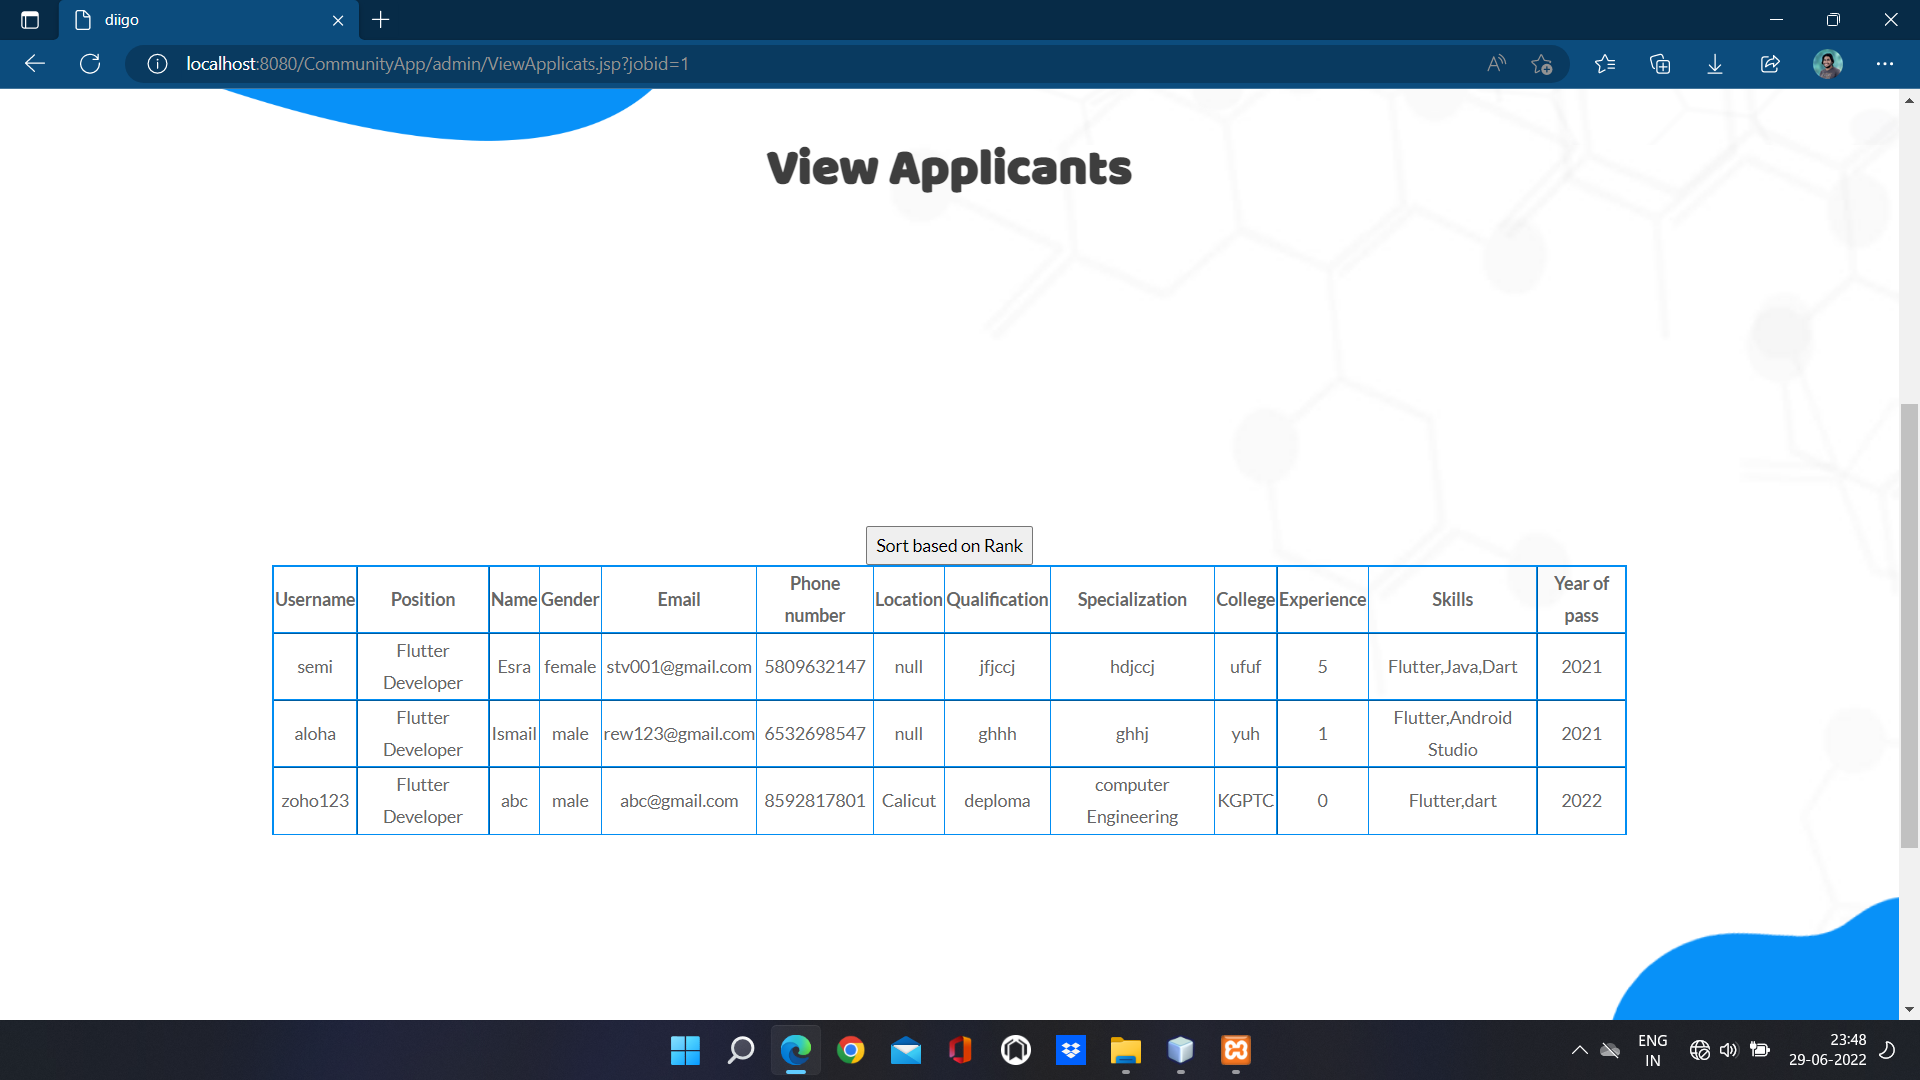
\includegraphics[scale=.20]{pcc3.png}
		\caption{VIEW APPLICANT PAGE BEFORE SORTING}
	\end{center}
\end{figure}
\begin{figure}[h]
	\begin{center}
		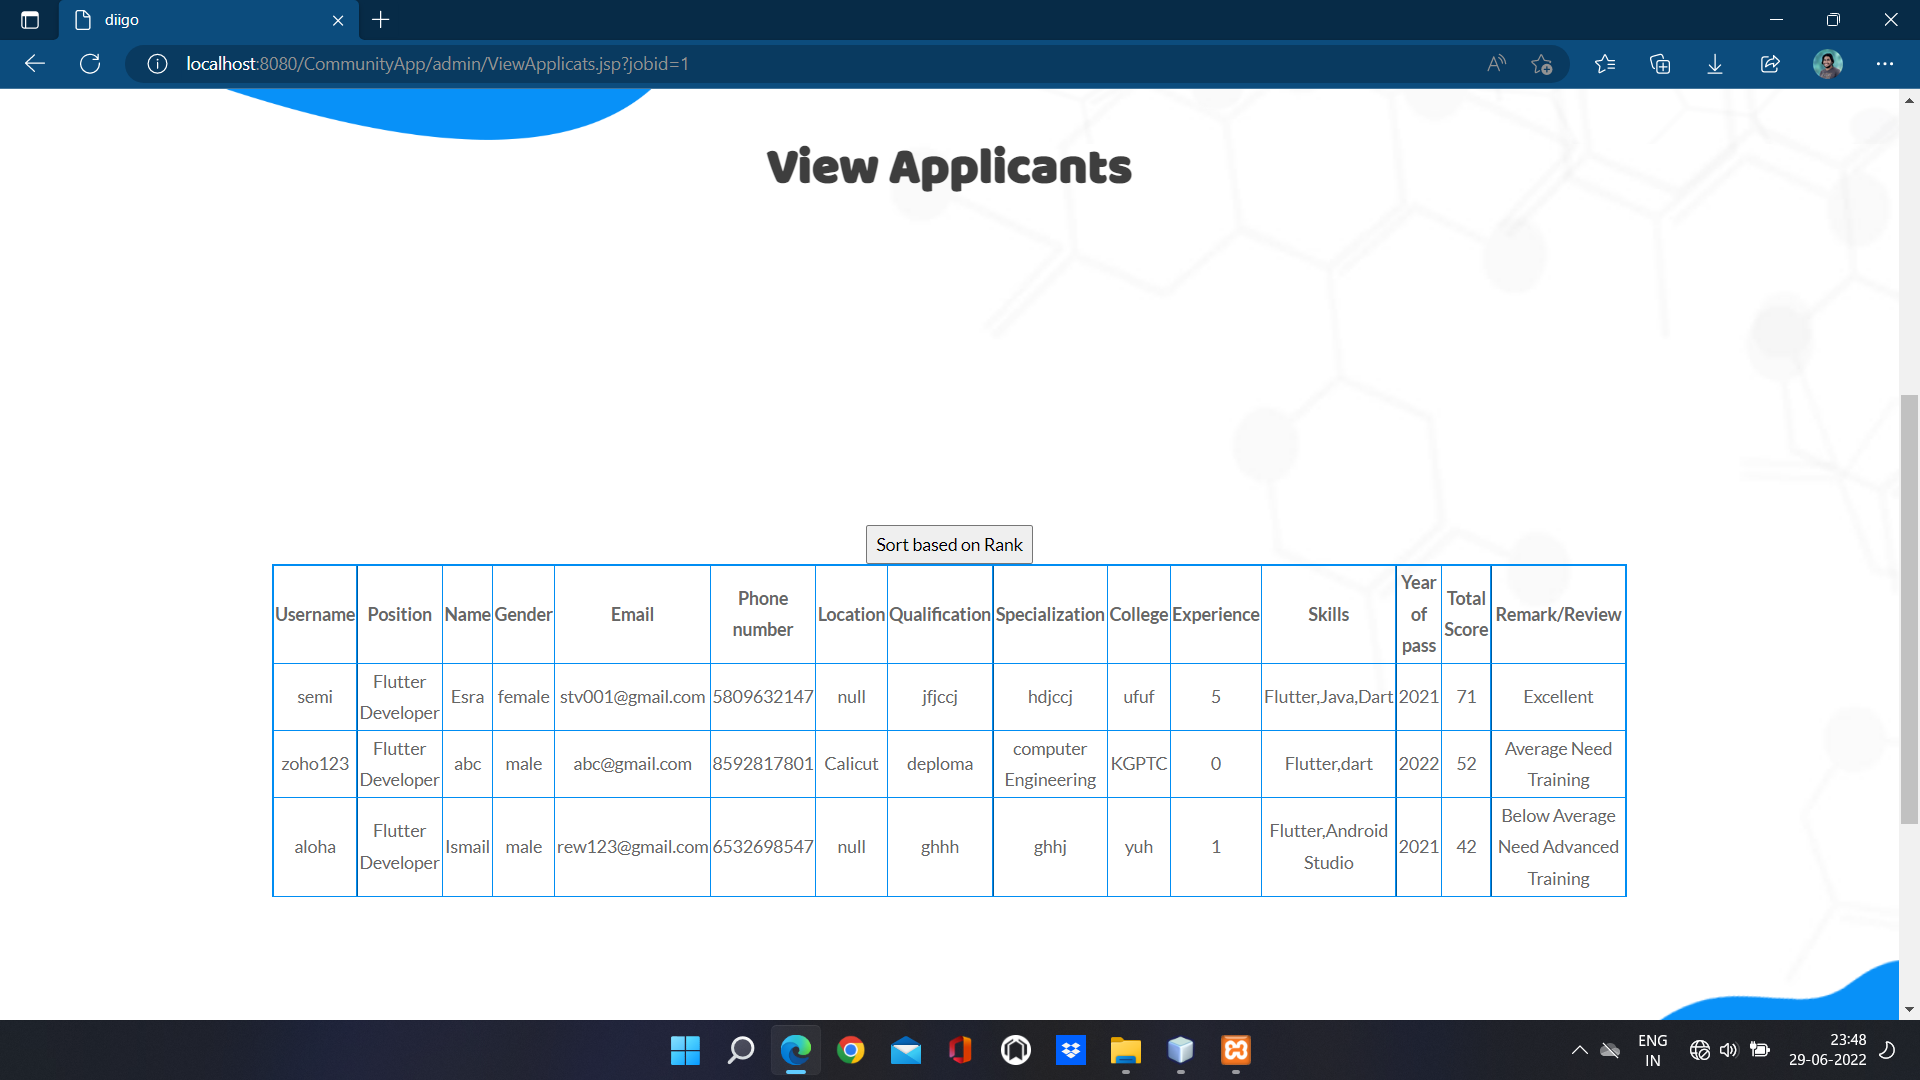
\includegraphics[scale=.20]{pcc4.png}
		\caption{VIEW  APPLICANT PAGE AFTER SORTING}
	\end{center}
\end{figure}

\chapter{SYSTEM TESTING}
\section{UNIT TESTING}
\begin{figure}[h]
	\begin{center}
		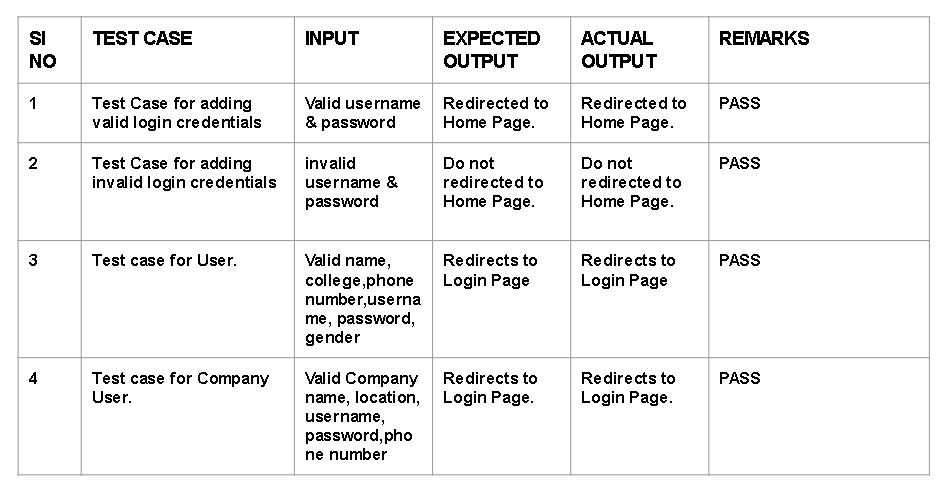
\includegraphics[scale=.61]{unit1.png}
		\vspace{.30 cm}
	\end{center}
\end{figure}
\begin{figure}[h]
	\begin{center}
		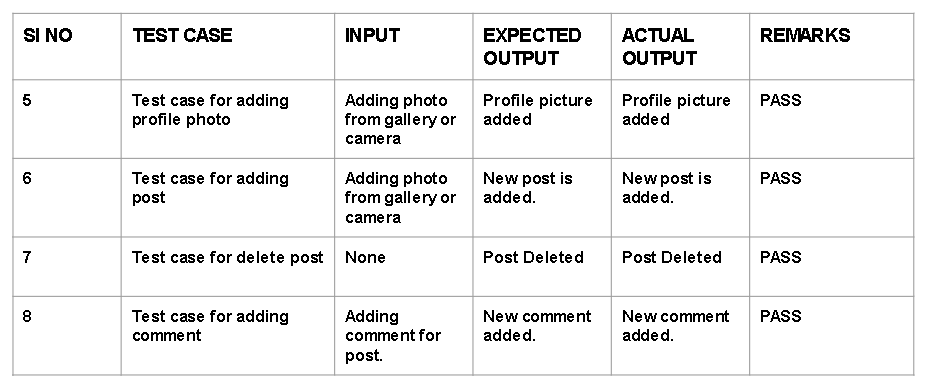
\includegraphics[scale=.62]{unit2.png}
		\vspace{.30 cm}
	\end{center}
\end{figure}
\section{INTEGRATION TESTING}
\begin{figure}[h]
	\begin{center}
		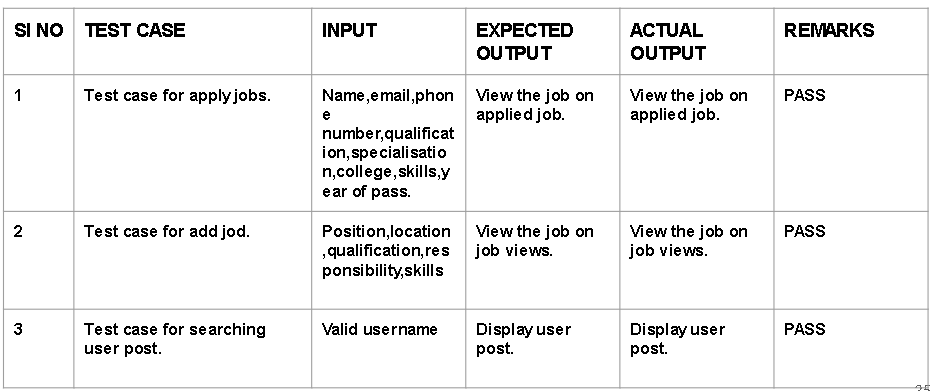
\includegraphics[scale=.60]{int1.png}
		\vspace{.30 cm}
	\end{center}
\end{figure}
\section{SYSTEM TESTING}
\begin{figure}[h]
	\begin{center}
		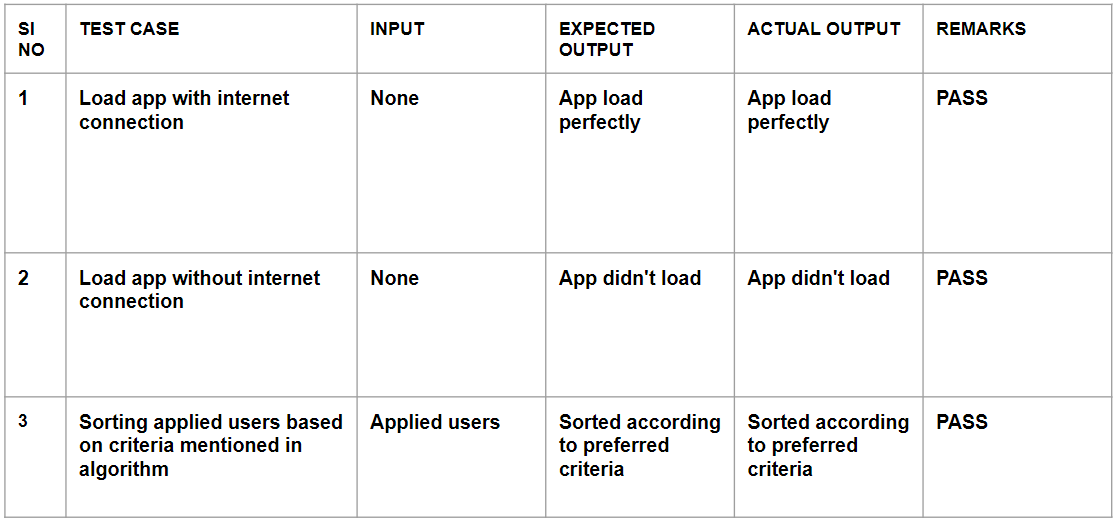
\includegraphics[scale=.56]{systemtest1.png}
		\vspace{.30 cm}
	\end{center}
\end{figure}
.
\chapter{CONCLUSION}
\hspace{01.5cm}ROUTES stands as a revolutionizing element in the sphere of recruitment. They act as a  
communication bridge between applicants and recruiters facilitating their requirements. This  
application helps organizations to have a greater exposure to the candidate pool and also job  
seekers facilitating wide search of jobs matching their interests. The android application provides  
flexibility to the jobseekers to view the openings and applied jobs.Our system develop an open community for employees and employers that reduces challenges in finding a desired  job   and filtering process that gives suitable candidates to the company based upon the qualifications and skill sets they mention. This application provides an enhanced user experience for both employer and jobseeker. It  
provides user friendly interface which facilitates in reaching wide range of audience.  
The application has achieved all the requirements that were initially set in the requirements  
gathering phase. 
\chapter{FUTURE SCOPES}
\hspace{01.5cm}This project is also developed for the future uses.Adding more security and some extra modules this system can be used in every platform.This project full fills the primary requirements of the job seekers and employers. It can be extended  
in several ways – We can provide suggestions and email updates for new job postings based  
on the job seekers search history. Since, the job seekers might be interested in building a strong  
Resume, we can provide tips and information for the same. We can also provide templates for  
building the Resumes which might interest most applicants. The mobile application is developed  
fulfilling the functionalities of job seeker, it can be extended to support functionalities of Employer  
as well.
\chapter{REFERENCES}
\textbf{1.http://www.wikipedia.com}\\
\textbf{2.https://msdn.microsoft.com}\\
\textbf{3.http://1000 projects.com}\\
\textbf{4.http://csharp corner.com}\\
\textbf{5.http://scribd.com}\\
\textbf{6.http://www.mayoclinic.org}\\
\textbf{7.https://citycentreclinic.com}\\

\end{document}